%%%%%%%%%%%%%%%%%%%%%%%%%%%%%%%%%%%%%%%%%%%%%%%%%%%%%%%%%%%%%%%%%%%%%%%%%%%%%%%%
%% Plantilla de memoria en LaTeX para la EIF - Universidad Rey Juan Carlos
%%
%% Por Gregorio Robles <grex arroba gsyc.urjc.es>
%%     Grupo de Sistemas y Comunicaciones
%%     Escuela de Ingeniería de Fuenlabrada
%%     Universidad Rey Juan Carlos
%% (muchas ideas tomadas de Internet, colegas del GSyC, antiguos alumnos...
%%  etc. Muchas gracias a todos)
%%
%% La última versión de esta plantilla está siempre disponible en:
%%     https://github.com/gregoriorobles/plantilla-memoria
%%
%% Para obtener PDF, ejecuta en la shell:
%%   make
%% (las imágenes deben ir en PNG o JPG)

%%%%%%%%%%%%%%%%%%%%%%%%%%%%%%%%%%%%%%%%%%%%%%%%%%%%%%%%%%%%%%%%%%%%%%%%%%%%%%%%

\documentclass[a4paper, 12pt]{book}
%\usepackage[T1]{fontenc}

\usepackage[a4paper, left=2.5cm, right=2.5cm, top=3cm, bottom=3cm]{geometry}
\usepackage{times}
\usepackage[utf8]{inputenc}
\usepackage[spanish]{babel} % Comenta esta línea si tu memoria es en inglés
\usepackage{url}
\usepackage[dvipdfm]{graphicx}
\usepackage{graphicx}
\usepackage{float}  %% H para posicionar figuras
\usepackage[nottoc, notlot, notlof, notindex]{tocbibind} %% Opciones de índice
\usepackage{latexsym}  %% Logo LaTeX
\usepackage[table,xcdraw]{xcolor}
\usepackage{array}
%\usepackage{graphicx} % Para usar \resizebox

\title{Memoria del Proyecto}
\author{Paula Sepúlveda Membrilla}

\renewcommand{\baselinestretch}{1.5}  %% Interlineado

\begin{document}

\renewcommand{\refname}{Bibliografía}  %% Renombrando
\renewcommand{\appendixname}{Apéndice}


%%%%%%%%%%%%%%%%%%%%%%%%%%%%%%%%%%%%%%%%%%%%%%%%%%%%%%%%%%%%%%%%%%%%%%%%%%%%%%%%
% PORTADA

\begin{titlepage}
\begin{center}
\includegraphics[scale=0.6]{img/URJ_logo_Color_POS.png}

\vspace{1.75cm}

\LARGE
ESCUELA DE INGENIERÍA DE FUENLABRADA
\vspace{1cm}

\LARGE
GRADO EN INGENIERÍA EN SISTEMAS AUDIOVISUALES Y MULTIMEDIA

\vspace{1cm}
\LARGE
\textbf{TRABAJO FIN DE GRADO}

\vspace{2cm}

\Large
EVOLUCIÓN DE PROYECTOS FOSS EN GITHUB

\vspace{2cm}

\large
Autor : Paula Sepúlveda Membrilla \\
Tutor : Dr. Gregorio Robles Martínez\\
\vspace{1cm}

\large
Curso académico 2023/2024

\end{center}
\end{titlepage}

\newpage
\mbox{}
\thispagestyle{empty} % para que no se numere esta pagina



%%%%%%%%%%%%%%%%%%%%%%%%%%%%%%%%%%%%%%%%%%%%%%%%%%%%%%%%%%%%%%%%%%%%%%%%%%%%%%%%
%%%% Para firmar
\clearpage
\pagenumbering{gobble}
\chapter*{}

\vspace{-4cm}
\begin{center}
\LARGE
\textbf{Trabajo Fin de Grado}

\vspace{1cm}
\large
Evolución de proyectos FOSS en GitHub

\vspace{1cm}
\large
\textbf{Autor :} Paula Sepúlveda Membrilla \\
\textbf{Tutor :} Dr. Gregorio Robles Martínez
\end{center}

\vspace{1cm}
La defensa del presente Proyecto Fin de Carrera se realizó el día \qquad$\;\,$ de julio de 2024, siendo calificada por el siguiente tribunal:


\vspace{0.5cm}
\textbf{Presidente:}

\vspace{1.2cm}
\textbf{Secretario:}

\vspace{1.2cm}
\textbf{Vocal:}


\vspace{1.2cm}
y habiendo obtenido la siguiente calificación:

\vspace{1cm}
\textbf{Calificación:}


\vspace{1cm}
\begin{flushright}
Fuenlabrada, a \qquad$\;\,$ de julio de 2024
\end{flushright}

%%%%%%%%%%%%%%%%%%%%%%%%%%%%%%%%%%%%%%%%%%%%%%%%%%%%%%%%%%%%%%%%%%%%%%%%%%%%%%%%
%%%% Dedicatoria

\chapter*{}
\pagenumbering{Roman} % para comenzar la numeracion de paginas en numeros romanos
\begin{flushright}
\textit{Cómo no vas a poder,}
\\\textit{si hay flores rompiendo el pavimento.}
\end{flushright}

%%%%%%%%%%%%%%%%%%%%%%%%%%%%%%%%%%%%%%%%%%%%%%%%%%%%%%%%%%%%%%%%%%%%%%%%%%%%%%%%
%%%% Agradecimientos

\chapter*{Agradecimientos}
%\addcontentsline{toc}{chapter}{Agradecimientos} % si queremos que aparezca en el índice
\markboth{AGRADECIMIENTOS}{AGRADECIMIENTOS} % encabezado 

Con la finalización de este proyecto llega el broche final de mi etapa universitaria, dejando atrás un período dulce y amargo,
donde los momentos complicados me han hecho crecer tanto en lo académico como en lo personal.

\\En primer lugar, quiero agradecer a mi familia el hecho de creer siempre en mí, llegar hasta aquí no habría sido posible sin vosotros,
gracias por vuestra paciencia. A mis padres, gracias por aguantar mi frustración y darme cordura en los momentos difíciles, por enseñarme
que con esfuerzo y dedicación puedo conseguir grandes cosas. A mi hermano, el mayor espectador de mi vida, tu apoyo incondicional me da alas.

\\Por otro lado, gracias a todos los amigos que me acompañan en el camino, tanto a los de siempre como a los recién llegados. Para mi la
amistad tiene un valor enorme y me hacéis sentirlo cada día. En especial gracias a esas amigas, que siempre están cerca cuando todo pesa un poco
más y que están dispuestas a celebrar mis logros de todo corazón, me hacéis sentir muy afortunada. Una mención especial para esas compañeras de universidad que se han convertido en amigas, siempre se quedará conmigo vuestra generosidad,
espero que nos quede mucho más por compartir.

\\Por último, gracias a mi tutor de proyecto, Gregorio Robles, por la inspiración y los conocimientos, y por tu ayuda durante la realización de este proyecto.

\\A todos ellos, gracias por el apoyo en esta etapa y por su aportación de distintas maneras a este Trabajo de Fin de Grado.

%%%%%%%%%%%%%%%%%%%%%%%%%%%%%%%%%%%%%%%%%%%%%%%%%%%%%%%%%%%%%%%%%%%%%%%%%%%%%%%%
%%%% Resumen

\chapter*{Resumen}
%\addcontentsline{toc}{chapter}{Resumen} % si queremos que aparezca en el índice
\markboth{RESUMEN}{RESUMEN} % encabezado

Este proyecto consiste en un análisis de repositorios FOSS\footnote{Free/Open Source Software} alojados en GitHub, con el
objetivo de estudiar la evolución del código abierto a lo largo de los años, así como de explorar la presencia de
posibles tendencias y/o patrones en este sector.

\\Para llevar acabo este análisis, se ha desarrollado una herramienta\footnote{https://github.com/paulasm13/TFG.git} que permite analizar todas las líneas de código presentes
en un repositorio de GitHub. Esta herramienta realiza un recorrido ascendente por todo el árbol del repositorio, analizando cada
archivo en cada subdirectorio. El análisis se basa en el uso del comando \textit{git blame}, lo que permite obtener datos relevantes
de cada versión del archivo investigando su historial de revisiones. 
Se ha hecho una selección de repositorios teniendo en cuenta diversos criterios, tales como el número de colaboradores y sus
contribuciones, la diversidad de lenguajes de programación utilizados, la relevancia del proyecto en la plataforma GitHub y su 
vigencia en la actualidad. Se han incluido tanto proyectos de reciente creación como aquellos con una larga trayectoria, para
proporcionar una visión más completa y representativa del estado actual del código abierto.

\\Empleando la herramienta desarrollada, se han recopilado datos interesantes como el lenguaje de programación empleado,
el autor y la fecha de creación cada la línea de código, así como el número de revisiones de cada archivo. Una vez recopilados los datos,
se ha procedido a su filtrado e inserción en una base de datos relacional organizada en tres tablas: \textit{Repositories}, \textit{Files}
y \textit{Code}. Para conseguir el objetivo de este proyecto, se han desarrollado diversas métricas e índices que permiten realizar un análisis
estadístico de los datos. Esta metodología se ha aplicado a la información recopilada, y los resultados del análisis se han representado de
manera gráfica, facilitando la comprensión de la evolución de los proyectos a lo largo de su historial de revisiones, y proporcionando una
visión clara de las tendencias y/o patrones que puedan existir.

%%%%%%%%%%%%%%%%%%%%%%%%%%%%%%%%%%%%%%%%%%%%%%%%%%%%%%%%%%%%%%%%%%%%%%%%%%%%%%%%
%%%% Resumen en inglés

\chapter*{Summary}
%\addcontentsline{toc}{chapter}{Summary} % si queremos que aparezca en el índice
\markboth{SUMMARY}{SUMMARY} % encabezado

This project consists of an analysis of FOSS\footnote{Free/Open Source Software} repositories hosted on GitHub, with the aim of studying the
evolution of open source over the years, as well as exploring the presence of possible trends and/or patterns in this sector.

\\To carry out this analysis, a tool\footnote{https://github.com/paulasm13/TFG.git} has been developed to analyse all the lines of code present in a GitHub repository. This tool performs a
bottom-up traversal of the entire repository tree, analysing each file in each subdirectory. The analysis is based on the use of the \textit{git blame}
command, which allows to obtain relevant data for each version of the file by investigating its revision history. A selection of repositories
has been made taking into account various criteria, such as the number of contributors and their contributions, the diversity of programming
languages used, the relevance of the GitHub platform and its current relevance. Both recently created projects and those with a long history
have been included, in order to provide a more complete and representative view of the current state of open source.

\\Using the tool developed, interesting data has been collected, such as the programming language used, the author and date of creation of each
line of code, as well as the number of revisions of each file. Once the data was collected, it was filtered and inserted into a relational database
organised into three tables: \textit{Repositories}, \textit{Files} and \textit{Code}. In order to achieve the objective of this project, various
metrics and indexes have been developed that allow a statistical analysis of the data to be carried out. This methodology has been applied to the
information collected, and the results of the analysis have been represented graphically, facilitating the understanding of the evolution of the
projects throughout their revision history, and providing a clear vision of the trends and/or patterns that may exist.

%%%%%%%%%%%%%%%%%%%%%%%%%%%%%%%%%%%%%%%%%%%%%%%%%%%%%%%%%%%%%%%%%%%%%%%%%%%%%%%%
%%%%%%%%%%%%%%%%%%%%%%%%%%%%%%%%%%%%%%%%%%%%%%%%%%%%%%%%%%%%%%%%%%%%%%%%%%%%%%%%
% ÍNDICES %
%%%%%%%%%%%%%%%%%%%%%%%%%%%%%%%%%%%%%%%%%%%%%%%%%%%%%%%%%%%%%%%%%%%%%%%%%%%%%%%%

% Las buenas noticias es que los índices se generan automáticamente.
% Lo único que tienes que hacer es elegir cuáles quieren que se generen,
% y comentar/descomentar esa instrucción de LaTeX.

%%%% Índice de contenidos
\tableofcontents 
%%%% Índice de figuras
\cleardoublepage
%\addcontentsline{toc}{chapter}{Lista de figuras} % para que aparezca en el indice de contenidos
\listoffigures % indice de figuras
%%%% Índice de tablas
\cleardoublepage
%\addcontentsline{toc}{chapter}{Lista de tablas} % para que aparezca en el indice de contenidos
\listoftables % indice de tablas


%%%%%%%%%%%%%%%%%%%%%%%%%%%%%%%%%%%%%%%%%%%%%%%%%%%%%%%%%%%%%%%%%%%%%%%%%%%%%%%%
%%%%%%%%%%%%%%%%%%%%%%%%%%%%%%%%%%%%%%%%%%%%%%%%%%%%%%%%%%%%%%%%%%%%%%%%%%%%%%%%
% INTRODUCCIÓN %
%%%%%%%%%%%%%%%%%%%%%%%%%%%%%%%%%%%%%%%%%%%%%%%%%%%%%%%%%%%%%%%%%%%%%%%%%%%%%%%%

\cleardoublepage
\chapter{Introducción}
\label{chap:introducción}
\label{sec:intro} % etiqueta para poder referenciar luego en el texto con~\ref{sec:intro}
\pagenumbering{arabic} % para empezar la numeración de página con números

En este capítulo se presenta la motivación que ha impulsado este Trabajo Fin de Grado,
proporcionando el contexto y las razones fundamentales para llevarla a cabo. A continuación, 
se define claramente el problema a resolver, especificando su alcance y relevancia, así como 
los objetivos que se desean alcanzar y las hipótesis planteadas al inicio del estudio.

\\Finalmente, se describe una visión general de cómo está organizado el documento y qué secciones lo componen.

\section{Motivación}
\label{sec:motivación}

La inspiración que me ha llevado a realizar este proyecto proviene de mi profesor y tutor, Gregorio Robles, quien me ha
motivado a adentrarme en el mundo del software libre (OSS, del inglés \textit{Open Source Software}).

\\El término software libre hace referencia al código diseñado de manera descentralizada y colaborativa, siendo
accesible para todo el público. Esto permite que cualquiera pueda utilizarlo, examinarlo, modificarlo y
redistribuirlo como considere conveniente.

\\La elección de código abierto aporta beneficios tales como un bajo coste, gran flexibilidad para
modificar el código fuente, así como un buen soporte proporcionado por parte de la comunidad.
Sin embargo, no existe una clara distinción entre el proceso de desarrollo y el de mantenimiento, lo cual resulta interesante
para la Ingeniería de Software al estudiar y explicar el funcionamiento de las interacciones que se llevan a cabo abiertamente.

\\Por lo tanto, la principal motivación de este Trabajo Fin de Grado es analizar el comportamiento de los proyectos de código abierto, los cuales se
desarrollan en una comunidad de usuarios que se comunican a través de distintas herramientas, teniendo como factor común Internet, lo que
permite guardar el registro de las actividades realizadas a lo largo del tiempo.

\\Además, este proyecto me ha brindado la oportunidad de adquirir conocimientos sobre minería de datos y desarrollar
habilidades para realizar un correcto análisis de los datos obtenidos.

\section{Definición del problema}
\label{sec:definición del problema}

El software libre permite a los desarrolladores realizar un completo análisis cuantitativo del
código y de todos los parámetros involucrados en su producción, debido a que están disponibles públicamente.
Al contar con datos de acceso público del desarrollo de software, permite llevar a cabo estudios estadísticos
para estudiar la evolución del software.

\\En todo este proceso, tiene gran importancia la utilización de un sistema de control de versiones, donde se permita
rastrear los cambios realizados en el pasado. De esta manera, se puede obtener un análisis de la estructura histórica
del código en base a sus distintas contribuciones, así como harían los arqueólogos estudiando una ciudad en base a sus
distintas construcciones.
Para el software libre esto tiene vital importancia, ya que debido a la falta de diseño, el mantenimiento del código
es una actividad relevante para evitar posible código obsoleto de desarrolladores que ya no participan en el proyecto.

\\Aunque la Ingeniería de Software es una disciplina que se ha consolidado a través de los años, actualmente
existen muy pocos análisis empíricos sobre la arqueología del software. La falta de estudios junto con el atractivo hacia el
desarrollo comunitario del software libre, así como la importancia para la Ingeniería de Software de modelar con datos empíricos,
nos impulsa a llevar a cabo este proyecto.

\section{Objetivos e hipótesis}
\label{sec:objetivos}

Nuestra hipótesis es que, mediante un estudio empírico de las prácticas de desarrollo de software, la aplicación de minería de datos
al proyecto, el análisis de su evolución a lo largo del tiempo y la correlación de datos, se pueden determinar y aplicar métricas
que demuestren que la longevidad y el mantenimiento del código son heterogéneos y varían entre los diferentes componentes de varios proyectos.

\\Por tanto, el objetivo del proyecto consiste en estudiar la evolución y propiedades de varios proyectos de software libre a través del estudio
empírico, y en aplicar un análisis estadístico de su código fuente.
Se estudia el comportamiento de los proyectos FOSS\footnote{Free/Open Source Software} más relevantes de GitHub, se identifican las fuentes de datos
que ofrecen de manera pública y se presenta una metodología para el análisis de los datos extraidos, datos interesantes entre los cuáles encontrampos 
la cantidad de colaboradores o los lenguajes de programación más utilizados.
De esta manera, se puede conocer mejor el fenómeno del software libre, el proceso de creación de software y cómo va evolucionando su mantenimiento,
se describe la mecánica de desarrollo de los movimientos de software libre.

\\En definitivas cuentas, este Trabajo Fin de Grado tiene como objetivo comprender la evolución de proyectos de software libre, así como interpretar los resultados obtenidos.

\section{Estructura de la memoria}
\label{sec:estructura}

A continuacion, se describe la estructura de la memoria, exponiendo el contenido de cada uno de los capítulos, proporcionando así
una guía organizada del Trabajo de Fin de Grado para una mejor lectura y comprension de este.

\begin{itemize}
  
  \item \textbf{Capítulo~\ref{chap:introducción}. Introducción}
  \\En este capítulo se describe la motivación que me ha llevado a realizar el Trabajo Fin de Grado, así
  como el contexto, la definición del problema y las distintas hipótesis que se han desarrollado. Además, se ha ofrecido una breve descripción de la estructura del proyecto.

  \item \textbf{Capítulo~\ref{chap:objetivos}. Objetivos}
  \\En este capítulo se describe el objetivo principal del Trabajo Fin de Grado, así como los objetivos específicos necesarios
  que van a guiar nuestro proyecto. Incluye una planificacion temporal de los objetivos mencionados. 
  
  \item \textbf{Capítulo~\ref{chap:estado-arte}. Estado del arte}
  \\En este capítulo se proporciona información detallada sobre el diseño, las características y los usos de cada
  una de las tecnologías y herramientas utilizadas en el proyecto.  
  
  \item \textbf{Capítulo~\ref{chap:diseño-implementacion}. Diseño e implementación}
  \\En este capítulo se detallan las fases que se han llevado a cabo para realizar el análisis de estudio. 
  Se describe la arquitectura general del proyecto, la mecánica de obtención y almacenamiento de los datos, y su posterior análisis empírico.

  \item \textbf{Capítulo~\ref{chap:resultados}. Resultados}
  \\En este capítulo se describen los resultados obtenidos tras analizar los datos recopilados en el análisis, y se 
  realiza una justificación de dichos resultados.
 
  \item \textbf{Capítulo~\ref{chap:conclusiones}. Conclusiones}
  \\En este capítulo se explican las conclusiones a las que se ha llegado, con su correspondiente justificación.
  Además, se mencionan los conocimientos adquiridos durante la duración de todo el grado universitario que se han aplicado en este proyecto, y los relacionados con el aprendizaje
  adquirido durante la realización de este estudio. Por último, se mencionan posibles mejoras que se pueden aplicar en el futuro.

\end{itemize}

%%%%%%%%%%%%%%%%%%%%%%%%%%%%%%%%%%%%%%%%%%%%%%%%%%%%%%%%%%%%%%%%%%%%%%%%%%%%%%%%
%%%%%%%%%%%%%%%%%%%%%%%%%%%%%%%%%%%%%%%%%%%%%%%%%%%%%%%%%%%%%%%%%%%%%%%%%%%%%%%%
% OBJETIVOS %
%%%%%%%%%%%%%%%%%%%%%%%%%%%%%%%%%%%%%%%%%%%%%%%%%%%%%%%%%%%%%%%%%%%%%%%%%%%%%%%%

\cleardoublepage % empezamos en página impar
\chapter{Objetivos} % título del capítulo (se muestra)
\label{chap:objetivos} % identificador del capítulo (no se muestra, es para poder referenciarlo)

En este capítulo, se definen los objetivos que guiarán la realización de este Trabajo de Fin de Grado.
Establecer objetivos claros y bien definidos es fundamental para asegurar una dirección precisa y coherente
a lo largo del desarrollo del proyecto.

\\Estos objetivos se dividen en dos categorías principales: el objetivo general,
que representa la meta global del trabajo, y los objetivos específicos, que son metas más concretas y detalladas necesarias
para alcanzar el objetivo general. 

\\Además, se presenta una planificación temporal que muestra la organización de las tareas a lo largo
del período de ejecución del proyecto, garantizando un avance ordenado y sistemático.

\section{Objetivo general} % título de sección (se muestra)
\label{sec:objetivo-general} % identificador de sección (no se muestra, es para poder referenciarla)

El objetivo general del proyecto consiste en investigar en profundidad la evolución y las características de proyectos de software libre
alojados en la plataforma de GitHub, mediante un estudio empírico detallado y la aplicación estadística de su código fuente. 
A través de este enfoque, se pretende obtener una comprensión íntegra de cómo el proyecto ha cambiado y se ha desarrollado a lo
largo del tiempo, identificando patrones, tendencias y características del código que puedan influir en su calidad, mantenibilidad y eficiencia.

\\Este Trabajo Fin de Grado no solo implica un análisis histórico, sino que también incluye la aplicacion de diversas métricas
para evaluar distintos aspectos del código fuente. 
Al combinar métodos empíricos con análisis estadísticos robustos, este proyecto busca proporcionar una visión detallada y objetiva
del comportamiento evolutivo del software.

\\Los resultados obtenidos ofrecen conclusiones y recomendaciones para la mejora continua del desarrollo del software libre,
contribuyendo al conocimiento en el campo de Ingeniería de Software que puede aplicarse en la toma de decisiones en proyectos futuros.

\section{Objetivos específicos}
\label{sec:objetivos-especificos}

Para lograr el objetivo general detallado en el proyecto se han establecido los siguientes objetivos específicos:
\begin{itemize}
  
  \item \textbf{Definición del problema y objetivos}
  \\Consiste en buscar y evaluar información sobre el contexto de trabajo, realizando una estimación de los
  costes de desarrollo software. Se piensa como desarrollar la programación de manera eficiente, y a su vez se realiza una selección de distintos
  repositorios de GitHub que resultan de especial interés para nuestro Trabajo Fin de Grado.

  \item \textbf{Programación}
  \\En esta fase del proyecto se desarrollan los scripts necesarios para extraer, almacenar y analizar los datos con
  el fin de conseguir los objetivos de este Trabajo Fin de Grado.
  
  \item \textbf{Recopilación de datos}
  \\En esta etapa se recopilan y almacenan los datos más relevantes para el posterior estudio del comportamiento
  de los repositorios seleccionados. También es importante realizar un preprocesado de los datos, lo que implica una
  normalización o estandarización de variables, así como una limpieza y transformación de datos según sea necesario.
  
  \item \textbf{Análisis estadístico}
  \\Tras la recopilación de los datos, se ajustan y configuran las métricas correspondientes para obtener
  distintas estadísticas sobre la evolución de los repositorios a lo largo del tiempo.

  \item \textbf{Evaluación e interpretación de los resultados}
  \\Una vez que se ha realizado un análisis estadístico, se realiza un análisis empírico y se representan 
  de manera gráfica los resultados obtenidos. Seguidamente, se interpretan los resultados obtenidos y se
  derivan conclusiones.
 
  \item \textbf{Documentación}
  \\En esta etapa se elaboran la documentación y los informes necesarios para la correcta entrega del Trabajo de Fin de Grado.

\end{itemize}


\section{Planificación temporal}
\label{sec:planificacion-temporal}

\begin{figure}
  \centering
  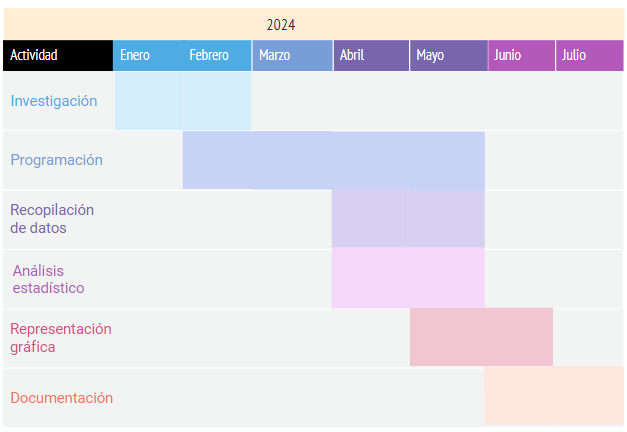
\includegraphics[width=14cm, keepaspectratio]{img/Diagrama_Gantt.png}
  \caption{Diagrama de Gantt}
  \label{fig:diagrama_gantt}
\end{figure}

El desarrollo de este proyecto abarca un período de siete meses, desde enero de 2024 hasta julio de 2024, con la realización de un trabajo diario que se lleva a cabo
de manera constante. En la figura~\ref{fig:diagrama_gantt} se observa el tiempo empleado en las diferentes fases del proyecto, donde se puede
observar que varias tareas se han solapado en algunos casos debido al avance en paralelo de distintas actividades.

\begin{itemize}

  \item \textbf{Enero}
  \\En este mes comienzo el desarrollo de este Trabajo Fin de Grado, cuando mi tutor Gregorio Robles me sugirió la idea del proyecto.
  Comienzan las reuniones donde se definen los objetivos correspondientes, y empiezo a documentarme para obtener los conocimientos
  necesarios para la realización del proyecto.
  \\Recopilo información acerca de los proyectos de código abierto y posibles repositorios de especial interés que están alojados en la plataforma de GitHub.
  A su vez, estudio la información que se puede obtener de las líneas de código mediante el comando \textit{git blame}, y qué análisis nos puede
  resultar de interés para estudiar la evolución de estos repositorios a lo largo de los años.

  \item \textbf{Febrero}
  \\Durante este mes sigo realizando la tarea de recopilación de información, pero además trabajo en paralelo con la tarea de programación. Comienzo a 
  desarrollar el código de programación basado en el comando \textit{git blame}, mediante el cual obtengo información interesante acerca de
  los cambios realizados en un archivo específico línea por línea. El comando \textit{git blame} nos proporciona información del autor de la
  línea de código, así como de la fecha de la revisión, del estado de esa línea y obviamente podemos ver también su contenido.
  
  \item \textbf{Marzo}
  \\En este mes me centro exclusivamente en la programación del código, desarrollando los scripts \textit{init.py} y \textit{git-blameall.py}. Estos scripts
  analizan un repositorio y un archivo respectivamente, con el objetivo de analizar línea a línea cada uno de los archivos de un repositorio, y guardan los datos recogidos en un archivo JSON.
  \\Al principio, se trabaja en realizar el análisis para un único archivo y finalmente se logra conseguir analizar un repositorio completo. Además, se estudia
  la opción de tener que analizar las distintas versiones de un archivo o unicamente la versión final, quedándonos con la segunda opción al ser mucho más eficiente y 
  conseguir obtener los datos que nos interesan.
  
  \item \textbf{Abril}
  \\Este mes tiene una gran carga de trabajo, al realizar en paralelo tres actividades distintas. Por una parte, sigo avanzando con la programación, mejorando los scripts \textit{init.py} y \textit{git-blameall.py}
  de manera que los datos pasan de guardarse en un archivo JSON a guardarse en una base de datos relacional organizada en tres tablas distintas relacionadas entre sí: \textit{Repositories}, \textit{Files} y \textit{Code} respectivamente.
  Esto requiere de un estudio previo para obtener los conocimientos necesarios sobre la utilización de \textit{MySQL} y el concepto de bases de datos relacionales. El hecho de almacenar los datos en bases de datos
  relacionales nos permite un posterior análisis de los datos de manera mucho más eficiente.

  \item \textbf{Mayo}
  \\Durante estas semanas la carga de trabajo sigue siendo muy alta, desarrollando cuatro actividades de manera paralela. Termino de desarrollar los archivos de programación, incluido entre ellos el script \textit{graphics.py}
  que tiene como finalidad poder obtener una representación gráfica de las métricas estudiadas. A su vez, termino de definir los índices y las métricas que se incluyen en este proyecto, para obtener estadísticas interesantes
  acerca de la evolución de cambios, número de autores o posible código obsoleto en un repositorio. Seguidamente, se recopilan los últimos datos de los repositorios elegidos para su análisis, todos ellos alojados en la plataforma
  de GitHub.

  \item \textbf{Junio}
  \\En esta etapa se elaboran las gráficas definitivas, y mientras tanto se empieza a escribir la memoria de nuestro proyecto.

  \item \textbf{Julio}
  \\En este último mes se termina de escribir la memoria y se realizan las correcciones oportunas por el tutor para poder realizar una correcta entrega del Trabajo de Fin de Grado.

\end{itemize}


%%%%%%%%%%%%%%%%%%%%%%%%%%%%%%%%%%%%%%%%%%%%%%%%%%%%%%%%%%%%%%%%%%%%%%%%%%%%%%%%
%%%%%%%%%%%%%%%%%%%%%%%%%%%%%%%%%%%%%%%%%%%%%%%%%%%%%%%%%%%%%%%%%%%%%%%%%%%%%%%%
% ESTADO DEL ARTE %
%%%%%%%%%%%%%%%%%%%%%%%%%%%%%%%%%%%%%%%%%%%%%%%%%%%%%%%%%%%%%%%%%%%%%%%%%%%%%%%%

\cleardoublepage
\chapter{Estado del arte}
\label{chap:estado-arte}

En este capítulo, se presentan las herramientas y bibliotecas usadas en el Trabajo Fin de Grado.
Esta exposicion nos da una visión de las tecnologías empleadas en el proyecto.

\section{Tecnologías y herramientas} 
\label{sec:tecnologias-herramientas}

\subsection{Python}
\label{subsec:python}

Python\footnote{\url{https://www.python.org/}} es un lenguaje de programación de alto nivel desarrollado por Guido Van Rossum a principios de 1989 en los Países Bajos.
Se trata de un lenguaje ejecutado directamente por un intérprete, que no requiere de una compilación previa, lo que facilita la detección y el manejo de errores. 
Es un lenguaje con una sintaxis clara y sencilla, por lo que resulta bastante atractivo para los desarrolladores por su fácil lectura, escritura y comprensión.
Además, Python se trata de un lenguaje multiplataforma, esto quiere decir que el mismo código puede utilizarse en distintos sistemas operativos al ser un lenguaje de código abierto,
lo que proporciona bastante versatilidad a los desarrolladores.

\\Incluye una gran cantidad de bibliotecas que proporcionan códigos para la visualización de datos con distintos gráficos, la creación de matrices o el procesamiento de imágenes. Esto permite
su amplia utilización en ámbitos muy distintos como las aplicaciones web, el desarrollo de software, la ciencia de datos o el machine learning (ML).

\\Ha experimentado un crecimiento significativo a lo largo de los años, pasando por distintas versiones, convirtiendose en uno de los lenguajes más populares y utilizados en la actualidad.

\subsection{GitHub}
\label{subsec:github}

GitHub\footnote{\url{https://github.com/}} es una plataforma de alojamiento de repositorios de código fuente que utiliza \textit{Git} como sistema de control
de versiones. Permite almacenar código y archivos en un servicio de la nube, de manera que los desarrolladores puedan colaborar en proyectos compartidos
manteniendo un seguimiento de la evolución del proyecto.

\\Linus Torvalds, un programador finlandés con gran importancia dentro del software libre, creó en 2005 su propio sistema de control de versiones llamado \textit{Git} para ser utilizado
en proyectos comerciales y de software libre. Posteriormente, en 2008, varios desarrolladores fundaron la plataforma GitHub, ofreciendo una interfaz fácil de utilizar que ha contribuido a la
popularización de \textit{Git}.

\\Es un sistema de control de versiones eficiente, fiable y compatible que se ha convertido en el estándar por excelencia para el desarrollo de software.

\subsection{MySQL}
\label{subsec:mysql}

MySQL\footnote{\url{https://mysql.com}} es un sistema de gestión de bases de datos considerado como uno de los más populares junto a Oracle y Microsoft SQL Server, sobre todo para entornos de desarrollo web.
Puede utilizarse en diferentes sistemas operativos con múltiples motores de almacenamiento para adaptarse a las necesidades de cada entorno. Sus puntos fuertes son la rapidez y la seguridad, ya que utiliza un
sistema de contraseñas que permite la verificación basada en host.

\\Uno de sus grandes beneficios es que cuenta con una gran comunidad con la que intercambiar dudas y conocimientos. Además, es escalable y fácil de aprender por lo que se convierte en una de las bases de datos
más utilizadas en la actualidad.

\subsection{LaTeX}
\label{subsec:latex}

LaTeX\footnote{\url{https://es.overleaf.com/}} es un sistema de composicion de textos o documentos formado por una colección de macros \textit{Tex}. Fue desarrollado
por Leslie Lamport en 1984, y en la actualidad se utiliza para la generación de artículos y libros científicos que incluyen, entre otros elementos, expresiones matemáticas.
Se utiliza para la composicion de tesis y libros técnicos, dado que la calidad tipográfica de los documentos realizados en LaTeX se considera adecuadas a las necesidades de
una editorial científica de primera línea, muchas de las cuales ya lo emplean.

\\\textit{Tex} es una mezcla entre procesador de textos y lenguaje de programación utilizado fundamentalmente para escribir documentos de contenido científico
y de gran calidad de impresión. Fue desarrollado por Donald E. Knuth en 1978, y actualmente hay implementaciones para todo tipo de ordenadores.
Es un sistema de tipografía muy popular en el entorno académico, especialmente entre las comunidades de matemáticos, físicos e informáticos.

\section{Bibliotecas} 
\label{sec:librerias}

\subsection{Pyodbc}
\label{subsec:pyodbc}

\textit{Pyodbc\footnote{\url{https://pypi.org/project/pyodbc/}}} es una biblioteca de Python que nos sirve para tener la integración de la comunicación con bases de datos de una manera sencilla. En el 
proyecto se ha utilizado para conectar nuestros scripts de Python con la base de datos alojada en MySQL.

\\Su funcionamiento consiste en conectarse a una base de datos mediante el comando \textit{connect()}, que nos devolverá una conexión. Una vez que tengamos
la conexión, se crea un cursor mediante la función \textit{cursor()}, con el cual podemos ejecutar \textit{querys()} para trabajar con los datos obtenidos. Una vez
que hayamos realizados las consultas oportunas, no hay que olvidarse de cerrar la conexión con la base de datos.

\subsection{Subprocess}
\label{subsec:subprocess}

La biblioteca \textit{subprocess}\footnote{\url{https://docs.python.org/es/3/library/subprocess.html}} permite ejecutar nuevos programas o comandos que se encuentran dentro de un script de Python a la vez que ejecutamos dicho script, es decir, ejecuta
procesos en segundo plano. Una de las capacidades más útiles consiste en que permite al usuario controlar las entradas, salidas e incluso los errores que genera el proceso hijo desde
dentro del código Python. Este modulo facilita la automatización de tareas y la integración de otros programas con el código de Python.

\subsection{Os}
\label{subsec:os}


La biblioteca \textit{os}\footnote{\url{https://docs.python.org/es/3.10/library/os.html}} permite usar funcionalidades dependientes del sistema operativo, como indica su nombre, por lo que es una biblioteca de gran tamaño y tiene muchos métodos.
Entre las funcionalidades más útiles se encuentran la de listar, crear y/o eliminar archivos y directorios, obtener el nombre de un archivo así como su directorio, obtener la extensión y tamaño de un archivo, así como obtener las fechas de creación, modificación
y/o de acceso de un archivo. En general, esta biblioteca facilita el trabajo con archivos y directorios independientemente de la plataforma, lo cual es bastante importante ya que debemos de tener en cuenta que los posibles usuarios de nuestro programa pueden tener distintos
sistemas operativos.

\subsection{Matplotlib}
\label{subsec:matplotlib}

\textit{Matplotlib}\footnote{\url{https://matplotlib.org/}} es una biblioteca muy completa de código abierto que se utiliza para crear visualizaciones estáticas, animadas e interactivas con Python.
Ha sido desarrollada por John Hunter en 2002, con el objetivo inicial de visualizar las señales eléctricas del cerebro de personas epilépticas.
Tras el fallecimiento de John Hunter, \textit{matplotlib} se ha ido mejorando a lo largo del tiempo por numerosos contribuidores de la comunidad de software libre.

\\Se trata de una herramienta muy completa, que permite generar visualizaciones de datos muy detalladas. Es posible crear trazados, histogramas, diagramas de barra y
cualquier tipo de gráfica para visualizar análisis estadísticos. 

\\El módulo \textit{Pyplot}\footnote{\url{https://matplotlib.org/stable/tutorials/introductory/pyplot.html}} propone varias funciones sencillas para añadir elementos tales como líneas, imágenes o textos
a los ejes de un gráfico. Su interfaz es muy intuitiva, lo que permite a los usuarios diseñar gráficos completamente personalizables con facilidad.

\subsection{Pandas}
\label{subsec:pandas}
\textit{Pandas} es una biblioteca de Python especializada en el manejo y análisis de estructuras de datos. Define nuevas estructuras de datos basadas en los arrays de la biblioteca \textit{NumPy} pero
con nuevas funcionalidades, nos permite leer y escribir fácilmente ficheros en bases de datos SQL y nos permite acceder a los datos mediante índices o nombres para filas y columnas.
Nos permite trabajar con tres estructuras de datos diferentes: estructura de una dimensión denominada \textit{series}, estructura de dos dimensiones o tablas denominada \textit{DataFrame} y estructura
de tres dimensiones o cubos llamada \textit{panel}.

\\El nombre \textit{«Pandas»} es en realidad una contracción del término \textit{«Panel Data»} para series de datos que incluyen observaciones a lo largo de varios periodos de tiempo. Se creó como herramienta
de alto nivel para el análisis en Python, y tiene la finalidad de evolucionar hasta convertirse en la biblioteca de manipulación de datos de código abierto más potente y flexible.

\subsection{Chardet}
\label{subsec:chardet}

\textit{Chardet} consiste en una adaptación para Python del detector de codificación de caracteres universal C++ de Mozilla. La detección de la codificación de caracteres es en realidad una detección del lenguaje
con dificultades, esto es especialmente útil cuando se trabaja con archivos de origen desconocido o múltiples fuentes que pueden tener diferentes codificaciones.

\\La forma más sencilla de utilizar esta biblioteca es mediante la funcion \textit{detect()}. Esta función toma un argumento de datos binarios y devuelve un diccionario que contiene la codificación de caracteres detectada
junto con el nivel de confianza de la detección. En el caso de utilizar esta biblioteca con archivos que contienen una gran cantidad de texto, lo recomendable es leer solo una parte del archivo y que se detenga tan pronto
como tenga la confianza suficiente para determinar su codificación. Esta biblioteca es útil en situaciones donde se reciben archivos históricos de múltiples fuentes con codificaciones no uniformes, como es el caso de nuestro proyecto.

\subsection{Pygments}
\label{subsec:pygments}

\textit{Pygments} consiste en una biblioteca de resaltado de sintaxis escrita en Python. Es una herramienta poderosa y flexible para resaltar la sintaxis de código fuente en múltiples lenguajes de programación y formatos
de salida, permite una personalización significativa para adaptarse a diferentes necesidades y preferencias.

\\De entre todas las funciones y herramientas que nos ofrece esta biblioteca, en este proyecto se han utilizado la función \textit{get\_lexer\_for\_filename} y la clase \textit{class pygment.lexer.name} con la finalidad
de adivinar el nombre del lexer, basado en el nombre y en el contenido del archivo. El \textit{lexer}, o también denominado \textit{analizador léxico} o \textit{tokenizer}, es un componente que convierte una secuencia de caracteres
en una secuencia de tokens, que se corresponden con unidades léxicas que representan estructuras significativas en el lenguaje de programación. Nos permite identificar y clasificar las diferentes partes del código fuente para poder
aplicar resaltado de sintaxis adecuado o para poder identificar el lenguaje de programación.


%%%%%%%%%%%%%%%%%%%%%%%%%%%%%%%%%%%%%%%%%%%%%%%%%%%%%%%%%%%%%%%%%%%%%%%%%%%%%%%%
%%%%%%%%%%%%%%%%%%%%%%%%%%%%%%%%%%%%%%%%%%%%%%%%%%%%%%%%%%%%%%%%%%%%%%%%%%%%%%%%
% DISEÑO E IMPLEMENTACIÓN %
%%%%%%%%%%%%%%%%%%%%%%%%%%%%%%%%%%%%%%%%%%%%%%%%%%%%%%%%%%%%%%%%%%%%%%%%%%%%%%%%

\cleardoublepage
\chapter{Diseño e implementación}
\label{chap:diseño-implementacion}
\label{sec:diseno}

A continuación, se proporciona una visión detallada del desarrollo de este proyecto, destacando los aspectos tanto técnicos como metodológicos que lo forman. Se describen en detalle las fases del proyecto, así como las métricas escogidas
con su debida justificación.

\\Exponer el diseño e implementación de nuestro proyecto permite a los lectores entender cómo se ha desarrollado este Trabajo Fin de Grado, además de proporcionarles la capacidad de contribuir o ampliar el proyecto.

\section{Arquitectura general} 
\label{sec:arquitectura-general}

En la figura~\ref{fig:arquitectura} se puede observar la arquitectura general del proyecto, que se compone de varias etapas interconectadas que permiten llevar a cabo la ejecución eficiente del mismo.

\begin{figure}
  \centering
  \includegraphics[width=14cm, keepaspectratio]{img/Arquitectura_general.png}
  \caption{Diagrama arquitectura general}
  \label{fig:arquitectura}
\end{figure}

\begin{figure}
  \centering
  \includegraphics[width=4cm, keepaspectratio]{img/Diagrama_Funcionamiento.png}
  \caption{Diagrama de funcionamiento}
  \label{fig:funcionamiento}
\end{figure}

En la figura~\ref{fig:funcionamiento} se presenta un diagrama de funcionamiento que nos permite comprender el desarrollo de la programación. 

\\Este diagrama consta del programa principal \texttt{init.py}, cuya función principal es clonar un repositorio de GitHub en nuestro directorio y poder recorrer cada uno de sus archivos y subdirectorios respectivamente.

\\Tras esto, se ejecuta el script \texttt{git\_blameall.py} con la finalidad de analizar línea a línea el código de cada archivo, recopilando diversos datos que se almacenan en varias tablas de la base de datos.

\\Finalmente, se ejecuta el script \texttt{graphics.py} con el objetivo de generar distintas gráficas que muestran los resultados de los análisis estadísticos y la aplicación de las métricas estudiadas previamente.

\section{Arquitectura específica} 
\label{sec:arquitectura-especifica}

En esta sección, se procede a describir más a fondo el funcionamiento de cada uno de los scripts que conforman nuestro proyecto.

\subsection{Programa inicial}
\label{subsec:programa-inicial}

El programa inicial se corresponde con el script \texttt{init.py}, ya que como indica el propio nombre, consiste en el script que inicia nuestro programa mediante el comando \textit{python3 init.py repo-url `name\_urlclone`}.
Se ejecuta a partir de la URL de un repositorio de GitHub, y entre sus diversas tareas esta la de ejecutar la función principal del programa \texttt{git\_blameall.py}, que como se indica posteriormente se trata del
programa principal. Sus funciones de manejo son las siguientes:

\begin{itemize}
  \item \texttt{request\_url()}. Al ejecutar el programa se pide introducir la URL de un repositorio de GitHub, mediante la cual podemos clonar el repositorio en nuestro directorio. De esta URL, se obtienen los valores del protocolo y procedencia del
  repositorio, de manera que mediante la función \texttt{check\_url()} se comprueba que se utilice un protocolo `https' y que el repositorio elegido sea propio de GitHub. Estos parámetros, junto con el nombre de usuario y del repositorio, nos permiten clonar
  el repositorio en nuestro directorio mediante la biblioteca \textit{subprocess} con la función \texttt{run\_url()}. Esta función además, ejecuta la función \texttt{get\_directory()}, y ésta a su vez la función \texttt{get\_path()}, que como el propio nombre
  indica obtienen el nombre del directorio y la ruta absoluta del directorio propio al repositorio clonado. Se ha utilizado una ruta absoluta frente a una relativa porque aporta claridad para evitar conflictos entre directorios ambiguos dentro del mismo repositorio,
  además de proporcionar independencia frente al lugar en el que se ejecute el script.

  \item \texttt{remove\_excluded()}. La finalidad de esta función consiste en clasificar archivos o directorios que no pueden ser soportados por el comando \textit{git blame} para ser posteriormente eliminados del repositorio clonado, por lo que 
  se descartan los archivos que tienen las siguientes extensiones [``.png", ``.jpg", ``.jpeg", ``.gif", ``.pdf", ``.exe", ``.dll", ``.ico", ``.db", ``.dat", ``.class", ``.o", ``.pyc", ``.mp3", ``.mp4", ``.wav", ``.avi", ``.bak", ``.tmp", ``.docx", ``.pptx", ``.zip",
  ``.tar.gz", ``.rar"] así como los siguientes directorios [``node\_modules", ``vendor", ``Pods"].
  
  \\Partiendo de las listas mencionadas anteriormente, se construye una función booleana para clasificar cada archivo o directorio a ser excluido del análisis, mediante el comando \texttt{file\_path.endwith()} se encuentran los archivos con la
  extensión correspondiente mientras que con la ayuda del separador de directorios específico de Windows \texttt{file\_path.split(os.path.sep)} obtenemos los posibles directorios a descartar. Una vez que tenemos los archivos y/o directorios que 
  tienen valor `True`, se realiza un recorrido ascendente por el árbol del repositorio clonado con la ayuda de \texttt{os.walk()} para eliminar cada objeto respectivamente. Al ejecutar el programa, se observan por pantalla los objetos que 
  se han eliminado así como la cantidad de objetos, esto ayuda a comprobar que se realiza un análisis de la cantidad correcta de archivos y/o directorios. 

  \item \texttt{remove\_empty\_files()}. Esta función tiene como finalidad eliminar archivos vacíos que se puedan encontrar en el directorio que se corresponde con el repositorio clonado, así como en todos sus subdirectorios.
  Toma como parámetro dicho directorio, y crea una lista inicialmente vacía que se utiliza para almacenar los nombres de los archivos eliminados. Mediante \texttt{os.walk()} se realiza un recorrido por todo el árbol del repositorio
  clonado e itera cada uno de sus archivos, para calcular su tamaño en bytes con el comando \texttt{os.path.getsize()}, y en caso de ser 0, se clasifica como un archivo vacío, y por lo tanto, se elimina mediante la función \texttt{os.remove()}
  y se añade a la lista de archivos eliminados. Finalmente, con la información incluida en la lista inicial, obtenemos información por pantalla acerca de que cantidad de archivos se han eliminado, y de cuáles son sus rutas y nombres respectivamente.
  
  \item \texttt{detect\_encoding()}. Esta función es una parte muy importante del código, ya que permite solucionar problemas de codificación al enfrentarse a cualquier tipo de archivo de datos. Tiene como objetivo adivinar el tipo de
  codificación del archivo pasado como parámetro, para ello realiza una lectura en bytes del archivo y mediante la biblioteca \textit{chardet} detecta la codificación del archivo.
  
  \item \texttt{convert\_to\_utf8()}. Esta función tiene como finalidad convertir en un archivo codificado en UTF-8 cada archivo que no esté codificado como tal, usando como parámetros el nombre del archivo a codificar y el tipo de codificación de dicho archivo.
  Se realiza una lectura en la codificación detectada anteriormente del archivo correspondiente, y se almacena su contenido en una variable. Este contenido se escribe en un archivo temporal, para posteriormente mediante la función \texttt{os.replace()}
  reescribir el archivo original con el contenido del archivo temporal, realizando así una conversión a la codificación UTF-8 de manera segura. 

  \item \texttt{get\_table1()}. A continuación, nos centramos en las tareas relacionadas con la base de datos. La primera tarea consiste en verificar la existencia de la base de datos que vamos a utilizar, esto se ha podido comprobar a través de la conexión a una base de datos
  \textit{`master'}, la cual nos proporciona la información necesaria, y en caso de que la base de datos denominada `Analysis\_Github\_Repository' no exista, se procede a crearla. El paso siguiente consiste en crear la tabla denominada \textit{Repositories}, previa comprobación de su existencia.
  
  \\Siguiendo en el ámbito de las bases de datos, utilizando la función \texttt{get\_table2()} se crea la tabla denominada \textit{Files} con las verificaciones necesarias y con una conexión previamente establecida a la base de datos \textit{Analysis\_Github\_Repository}.

  \item \texttt{read\_directory()}. Esta función es la más importante de todo el script, ya que integra y unifica la mayoria de las funciones descritas anteriormente. En primer lugar, toma como parámetro el nombre del directorio que se va a analizar y crea una lista con todos sus archivos y subdirectorios.
  De esta lista, descarta el directorio `.git' para el análisis pero teniendo en cuenta que no se puede eliminar, al contener información de vital importancia sobre el repositorio clonado, incluyendo su historial de versiones, su configuración así como sus objetos. Tras esto, el procedimiento a seguir consiste
  en recorrer el árbol del repositorio, clasificando cada objeto de la lista según sea un archivo o un subdirectorio. 
  
  \\En caso de ser un archivo, se construye y ejecuta el comando \textit{git log} para obtener el historial de versiones del archivo. Si el comando falla, se imprime un mensaje de error y se continúa con el siguiente archivo, pero si el comando se ejecuta con éxito, se cuenta el número de commits del archivo, y 
  en caso de tener un número de commits superior a 0, se ejecuta la función principal del script \texttt{git\_blameall.py}. Mientras tanto, se ejecutan las funciones relacionadas con la codificación original del archivo, y se convierte a UTF-8 en caso de ser necesario. Así como también se adivina el lenguaje de
  programación del archivo mediante la biblioteca \textit{Pygments}. En caso de ser un subdirectorio, se muestra su nombre por pantalla y se invoca esta función recursivamente, con el objetivo de analizar todos los archivos del repositorio clonado.
  
  \\Mediante una conexión a la base de datos se realiza la inserción de datos obtenidos en esta función. Primero se utiliza la función \texttt{insert\_repo\_data()}, que inserta en la tabla \textit{Repositories} el nombre del repositorio clonado así como su índice correspondiente. Posteriormente se ejecuta la función
  \texttt{insert\_files\_data()} que se encarga de insertar en la tabla \textit{Files} el nombre, ruta, ID y número de revisiones de cada archivo respectivamente. También se ejecuta la función \texttt{insert\_files\_language()}, que inserta el lenguaje de cada archivo dentro de la tabla \textit{Files}.
\end{itemize}

\subsection{Programa principal}
\label{subsec:programa-principal}

El programa principal se corresponde con el script \texttt{git\_blameall.py}, que consiste en el script que analiza cada fichero utilizando distintos comandos de git. Su objetivo principal es obtener datos interesantes del historial de cambios propio de cada archivo, que se utilizarán posteriormente para estudiar y 
analizar la evolución del repositorio. Sus funciones de manejo son las siguientes:
\begin{itemize}
  \item \texttt{parse\_chunk\_header()}. En el contexto de Git y las diferencias (\textit{diffs}) entre un archivo, un \textit{chunk} se corresponde con la sección de un archivo que ha cambiado entre dos revisiones, por lo que esta es la forma que tiene Git de mostrar las posibles diferencias. Cada \textit{chunk} 
  contiene una cabecera que indica dónde se encuentra el cambio realizado y cuántas líneas se han añadido y/o eliminado, y también las líneas de código modificadas con prefijos que indican respectivamente si la línea ha sido añadida o eliminada.
  
  \\Esta función analiza la cabecera del \textit{chunk} con el objetivo de extraer información sobre las líneas afectadas. Se obtiene una lista con los valores del índice de la línea inicial en la versión original del archivo donde comienza el cambio (\textit{origL}), el número de líneas eliminadas en la versión original
  del archivo (\textit{del\_N}), el índice de la línea inicial en la nueva versión del archivo donde comienza el cambio (\textit{newL}) y el número de líneas añadidas en la nueva versión del archivo (\textit{add\_N}). En caso de que no se puedan obtener los valores de (\textit{del\_N}) o (\textit{add\_N}), serán
  considerados `1' por defecto. En conclusión, esta función nos retorna las posiciones y números de líneas afectadas.
  
  \item \texttt{get\_initial\_version()}. El objetivo de esta función consiste en obtener el contenido inicial de un archivo en una revisión específica de Git, toma como parámetros el \textit{hash} de la primera revisión del archivo y el nombre del archivo en cuestión. Cuando se habla de \textit{hash} se refiere al identificador
  de cada revisión/commit realizada sobre el archivo. Teniendo en cuenta estos parámetros, construye el comando \textit{git show} y se ejecuta, obteniendo como salida el contenido inicial del archivo, que almacena línea a línea en la lista \textit{lines}.

  \item \texttt{find\_index()}. Esta función tiene como parámetros una lista con todas las líneas del archivo inicial, cada una de ellas con su información correspondiente, además del número de líneas que se deben de avanzar desde la línea de referencia. El procedimiento de la función se basa en recorrer una a una las líneas que
  permanecen en la actualidad (vivas) hasta que el número de líneas a avanzar sea 0, teniendo en cuenta que se considera una línea viva aquella que no tiene una fecha de fin y que fue introducida en una revisión distinta a la actual. Tiene como objetivo encontrar el índice correcto de la posición donde se debe de insertar o eliminar
  alguna línea.
    
  \item \texttt{main()}. Esta es la función más importante de todo el script, donde se integran todas las anteriores. Tiene como objetivo analizar todas las revisiones de un archivo de un repositorio de Git y registrar información sobre los cambios producidos en una base de datos SQL Server. En primer lugar, construye y ejecuta
  el comando \textit{git rev-list}, obteniendo como salida una variable denominada \textit{hashes} con todas las revisiones que ha sufrido ese archivo y sus respectivos identificadores, ordenadas cronológicamente de la más antigua a la más actual. Seguidamente, ejecuta el comando \textit{git log} para obtener las fechas y los autores
  de cada una de las revisiones, que se guardan en la variable \textit{date\_author}. Realiza la comprobación de que el número de revisiones obtenido coincida con la longitud de \textit{date\_author}, y crea una lista de objetos \textit{struct} denominada \textit{revs} que contiene la información de cada revisión de la siguiente manera:
  (hash, fecha, autor). Según el procesamiento de líneas indicado, recorre cada línea de código de la versión inicial del archivo, y se guardan en la lista \textit{ALL\_LINES} como objetos de tipo \textit{struct}.
  
  \\Una vez que se ha obtenido la versión inicial del archivo, se procesa cada una de sus revisiones desde la más reciente hasta la más antigua. Se utiliza el comando \textit{git diff} para obtener las posibles diferencias entre revisiones, y se procesa cada una de sus líneas resultantes en función del tipo de línea obtenida: si es una
  cabecera de chunk (\textit{@@}), se extrae la información correspondiente sobre el chunk llamando a la función \texttt{parse\_chunk\_header()}, y si es una línea eliminada (\textit{-}) o añadida (\textit{+}), encuentra el índice correspondiente en \textit{ALL\_LINES} usando la función \texttt{find\_index()}, verifica la modificación
  en la revisión actual e inserta los cambios en la base de datos. También se insertan en la base de datos las líneas vivas que se encuentran en la versión más actual, es decir, las líneas que no se han modificado nunca desde la versión inicial del archivo.
  
  \\En conclusión, esta función se centra en guardar las líneas que han sufrido cambios durante las revisiones así como aquellas que no se han cambiado desde la versión inicial.

  \item \texttt{print\_so\_far()}. La finalidad de esta función es manejar la conexión con la base de datos, verificar y crear la tabla \textit{Code} en caso de que no exista, e insertar cada una de las líneas mencionadas anteriormente en esta tabla.
\end{itemize}

\subsection{Obtención de gráficos}
\label{subsec:programa-graficos}

La obtención de gráficos se consigue con la ejecución del script \texttt{graphics.py}. Realizando consultas a la base de datos, utilizando en ellas distintos métodos, obtengo los datos necesarios en cada caso para poder aplicar las métricas e índices
correspondientes. Tras esto, y con ayuda de la biblioteca \textit{matplotlib}, se obtienen los resultados y se interpretan de manera gráfica.

\\Este script tiene varias funciones para obtener distintas gráficas, las cuales se desarrollan de manera muy mecánica puesto que siguen el mismo procedimiento. Primero, se realiza una consulta y extracción en la base de datos, obteniendo así los datos
correspondientes, que se guardan en un elemento DataFrame. Tras esto, se realizan los ajustes y cálculos correspondientes según las necesidades de cada función, y por último, se lleva a cabo una representación gráfica de los resultados.

\section{Fases del proyecto} 
\label{sec:fases-proyecto}

En esta sección se desglosan las distintas fases del proyecto, describiendo el desarrollo de cada una de ellas.

\subsection{Recopilación de datos}
\label{subsec:recopilacion}

En esta etapa del proyecto, se tiene como objetivo identificar proyectos de software libre que resulten interesantes para estudiar su evolución. Por lo que se realiza una exhaustiva búsqueda, revisando gran variedad de artículos e
información, para obtener una serie de repositorios que cumplan los siguientes criterios: que sean proyectos FOSS\footnote{Free/Open Source Software}, que estén alojados en la plataforma de GitHub y que proporcionen datos que resulten interesantes
para analizar su evolución a lo largo de los años.

\\Tras estudiar las distintas posibilidades, se han elegido los principales repositorios de los proyectos de la tabla~\ref{tab:repositorios} para estudiar su evolución a lo largo del tiempo. En la selección se han considerado factores como el número de colaboradores y/o
su variación a lo largo de los años, la diversidad de lenguajes de programación, la relevancia del proyecto en la plataforma GitHub y en la actualidad, así como que sean tanto proyectos de nueva creación como proyectos de larga trayectoria. Se puede observar una breve descripción
de cada repositorio elegido en la tabla~\ref{tab:repositorios-descripción}.

\begin{table}
 \begin{center}
  \begin{tabular}{ | l | c | c | c | c |} % tenemos tres colummnas, la primera alineada a la izquierda (l), la segunda al centro (c) y la tercera a la derecha (r). El | indica que entre las columnas habrá una línea separadora.
    \hline
    \textbf{Proyecto}          & \textbf{Repositorio}           & \textbf{Nº archivos}           & \textbf{Contribuidores}  & \textbf{Año 1ª revisión}             \\ \hline % el hline nos da una línea vertical
    Jupyter                    & Notebook                       & 265                            & 557                      & 2015                                 \\ \hline
    Vue                        & Core                           & 660                            & 486                      & 2018                                 \\ \hline
    Kanaries                   & Rath                           & 680                            & 17                       & 2019                                 \\ \hline
    CodeEdit                   & CodeEdit                       & 637                            & 123                      & 2022                                 \\ \hline
    HPC-AI Tech                & Open-Sora                      & 294                            & 49                       & 2024                                 \\ \hline
    Wulkano                    & Kap                            & 227                            & 52                       & 2016                                 \\ \hline
    Moment.js                  & Luxon                          & 148                            & 232                      & 2015                                 \\ \hline
    Ant Design Team            & Ant-design-pro                 & 152                            & 321                      & 2017                                 \\ \hline
    Nba-go                     & Nba-go                         & 52                             & 14                       & 2017                                 \\ \hline
    Chaoss                     & grimoriolab-perceval           & 514                            & 40                       & 2015                                 \\ \hline
    OpenUBL                    & ublhub                         & 390                            & 4                        & 2020                                 \\ 
    \hline
  \end{tabular}
  \caption{Selección de repositorios para el análisis}
  \label{tab:repositorios}
 \end{center}
\end{table}

\begin{table}
  \begin{center}
   \begin{tabular}{ | l | p{12cm} |} % p mide el ancho de la columna y permite el salto de línea de forma automática
     \hline
     \textbf{Repositorio}    & \textbf{Descripción}                                                                                                                  \\ \hline % el hline nos da una línea vertical
     Notebook               & Aplicación interactiva para escribir y ejecutar código, crear visualizaciones y documentar código en un formato de cuaderno.           \\ \hline
     Core                   & Herramienta de JavaScript progresiva y de adopción incremental para crear interfaces de usuario en la web.                             \\ \hline
     Rath                   & Plataforma de nueva generación automatizada para el análisis exploratorio y la visualización de datos.                                 \\ \hline
     CodeEdit               & Editor de código para macOS que proporciona una experiencia similar a TextEdit pero con características similares a Xcode.             \\ \hline
     Open-Sora              & Plataforma dedicada a la producción eficiente de vídeo de alta calidad.                                                                \\ \hline
     Kap                    & Grabador de pantalla construido con tecnología web.                                                                                    \\ \hline
     Luxon                  & Biblioteca para trabajar con fechas y horas en JavaScript.                                                                             \\ \hline
     Ant-design-pro         & Plantilla preconstruida en React que facilita el desarrollo de interfaces de usuario para aplicaciones empresariales.                  \\ \hline
     Nba-go                 & Herramienta para fanáticos de la NBA, permite ver la NBA en vivo así como los resultados y los datos de los jugadores.                 \\ \hline
     grimoriolab-perceval   & Perceval es un módulo de Python para recuperar datos de repositorios relacionados con el desarrollo de software.                       \\ \hline
     ublhub                 & Crea y envía comprobantes electrónicos (XML) a la SUNAT (Superintendencia Nacional de Aduanas y de Administración Tributaria) de Perú. \\ 
     \hline
   \end{tabular}
   \caption{Breve descripción de cada repositorio}
   \label{tab:repositorios-descripción}
  \end{center}
 \end{table}

 \\Una vez elegidos los repositorios a analizar, se lleva a cabo la recopilación de los datos, que se trata de una tarea crucial para cualquier proyecto de análisis o minería de datos. En esta fase, recogemos los siguientes datos para su posterior 
almacenamiento:

\begin{itemize}
  \item \textbf{Repo\_Name}. Como el propio nombre indica, se refiere al nombre de cada repositorio. De manera que se pueda realizar una clasificación de líneas o archivos según pertenezcan a un repositorio concreto.
  \item \textbf{Repo\_ID}. Al realizar un análisis de varios repositorios, cada repositorio se identifica con un ID correspondiente. De esta forma, es más sencillo identificar los datos y podemos llevar a cabo la funcionalidad
  de tabla de datos relacional.
  \item \textbf{File\_ID}. Al igual que cada repositorio se identifica con su propio ID, se hará lo mismo con cada archivo. De manera que se puedan clasificar las líneas de código pertenecientes a un archivo concreto.
  \item \textbf{File\_Name}. Este valor se corresponde con el nombre del archivo que se va a analizar.
  \item \textbf{File\_Path}. Este campo se corresponde con la ruta donde se encuentra el archivo que se está analizando, de manera que se pueda localizar en el repositorio clonado.
  \item \textbf{File\_Language}. Este dato se corresponde con el lenguaje del archivo que se está analizando. El lenguaje se ha identificado mediante la biblioteca \textit{Pygments}, clasificandose como `Archivo de datos' aquel
  archivo al que no se le ha podido identificar su lenguaje de programación, y que puede almacenar diversos datos como texto plano, datos binarios, etc. 
  \item \textbf{Commits}. Este dato se corresponde con el número de revisiones que se ha realizado sobre el archivo que se está analizando. Cada 'commit' se corresponde con la acción que se realiza para guardar los cambios realizados en los archivos de 
  un repositorio. El conjunto de todos estos commits forman el historial de revisiones de cada repositorio, por lo que el número de commits o revisiones nos puede indicar la frecuencia de actualizaciones de un proyecto.
  \item \textbf{Code\_ID}. Cada línea que se guarda en la base de datos se identifica con su propio ID.
  \item \textbf{Author\_Start}. Este valor se corresponde con el autor de la línea de código correspondiente, es decir, aquella persona que desarrolló esta línea por primera vez.
  \item \textbf{Date\_Start}. Este dato se corresponde con la fecha de creación de la línea de código correspondiente.
  \item \textbf{Author\_End}. Este valor se corresponde con el desarrollador que eliminó la línea de código correspondiente.
  \item \textbf{Date\_End}.   Este dato se corresponde con la fecha en la que la línea de código ha sido eliminada.
  \item \textbf{Longevity}. Teniendo en cuenta la fecha de creación y la posible fecha de fin de cada línea de código, se realiza un cálculo de los días de vida que tiene la línea de código. El resultado de este cálculo se guarda en esta variable.
  \item \textbf{Comment\_Boolean}. Se clasifica como `1' la línea de código que se corresponde con un comentario de línea, teniendo en cuenta los distintos comentarios en los diversos lenguajes de programación. Así como se identifica como `0' en el
  caso contrario, es decir, en caso de no ser un comentario de línea.
  \item \textbf{Words\_Count}. Este dato se corresponde con el cálculo de las palabras que forman cada línea de código. 
  \item \textbf{Code}. En esta variable se inserta la línea de código en cuestión que se está analizando.
\end{itemize}

\subsection{Almacenamiento de datos}
\label{subsec:almacenamiento}

Una vez que se recopilan los datos mencionados en el apartado anterior, la siguiente tarea consiste en su almacenamiento en una base de datos. Este almacenamiento se realiza en una base de datos relacional, que consiste en una colección de información que organiza datos
en relaciones predefinidas, en la que los datos se almacenan en una o más tablas de columnas y filas, lo que facilita su visualización y la comprensión de cómo se relacionan las diferentes estructuras de datos entre sí. Las tablas se relacionan con otras tablas mediante una
relación de clave primaria o de clave foránea, estableciendo relaciones de uno a uno, uno a muchos, o muchos a muchos entre tablas. Una clave primaria es una columna o un conjunto de columnas en una tabla cuyos valores identifican de forma exclusiva una fila de la tabla, mientras
que los valores de la clave foránea se corresponden con los valores de la clave primaria de otra tabla. Los principales beneficios de este modelo de base de datos son evitar la duplicidad de los registros y garantizar la integridad referencial de los datos, proporcionando así una
manera intuitiva de representar los datos y un acceso fácil a datos relacionados. Este modelo de bases de datos garantiza las propiedades \textit{ACID}, que consisten en atomicidad, que garantiza que los datos no se modifican en caso de producirse un error en alguna parte de la
transacción; consistencia, que garantiza que los datos cumplan con las restricciones de integridad; aislamiento, permitiendo que las operaciones de realizadas sobre la base de datos sean indendientes y que no afecten las unas a las otras; y durabilidad, que proporciona la persistencia
de las operaciones realizadas sobre los datos de manera que todos los cambios sean permanentes.

\\Las bases de datos relacionales se caracterizan por utilizar el lenguaje de consulta SQL, por lo que también se denominan bases de datos SQL. Mediante este lenguaje se realizan las operaciones básicas de interacción con la base de datos, definiendo a continuación las que han sido
utilizadas en este proyecto:
\begin{itemize}
  \item \textbf{CREATE DATABASE}. Se corresponde con la sentencia utilizada para crear la base de datos \textit{Analysis\_GitHub\_Repository}.
  \item \textbf{CREATE TABLE}. Como el propio nombre indica, esta sentencia o query se utiliza para crear una tabla dentro de la base de datos. Se deben de especificar los campos que contenga la tabla, así como sus tipos, sus claves primarias o foráneas, o incluso se pueden restringir
  algunos campos para que sean válidos o no los valores \textit{NULL}.
  \item \textbf{INSERT INTO}. Esta sentencia se utiliza para insertar valores en una tabla existente en la base de datos. Se deben de especificar los valores a insertar y el propio nombre de la tabla.
  \item \textbf{SELECT}. Esta sentencia aporta diferentes funcionalidades, siendo una de ellas la verificación de la existencia de una tabla de la base de datos, con el objetivo de poder crear la tabla correspondiente en caso de ser necesario así como solamente tener acceso a ella
  en caso de ya estar creada. Por otro lado, se utiliza esta sentencia para obtener distintos datos de las tablas de la base de datos, en función de los campos que consideremos necesarios para calcular la métrica correspondiente y representar su respectivo gráfico resultante.
\end{itemize}

\\En la figura~\ref{fig:entidad-relacion}, se observa un diagrama de entidad relación (DER) que consiste en una herramienta para representar de manera simplificada cómo se ha organizado la información de la base de datos \textit{Analysis\_GitHub\_Repository}. Esta base de datos se compone de tres tablas
distintas denominadas \textit{Repositories}, \textit{Files} y \textit{Code}. De la tabla \textit{Repositories} se establece una relación de uno a muchos, puesto que dentro de un repositorio se organizan diversos archivos, por lo que la clave primaria del ID correspondiente
al repositorio pasa a ser la clave foránea de la tabla \textit{Files}. Sucede lo mismo desde la tabla \textit{Files} hacia la tabla \textit{Code}, ya que de un archivo se obtienen múltiples líneas de código, por lo que la clave primaria del ID correspondiente a cada archivo
pasa a ser la clave foránea en la siguiente tabla.

\begin{figure}
  \centering
  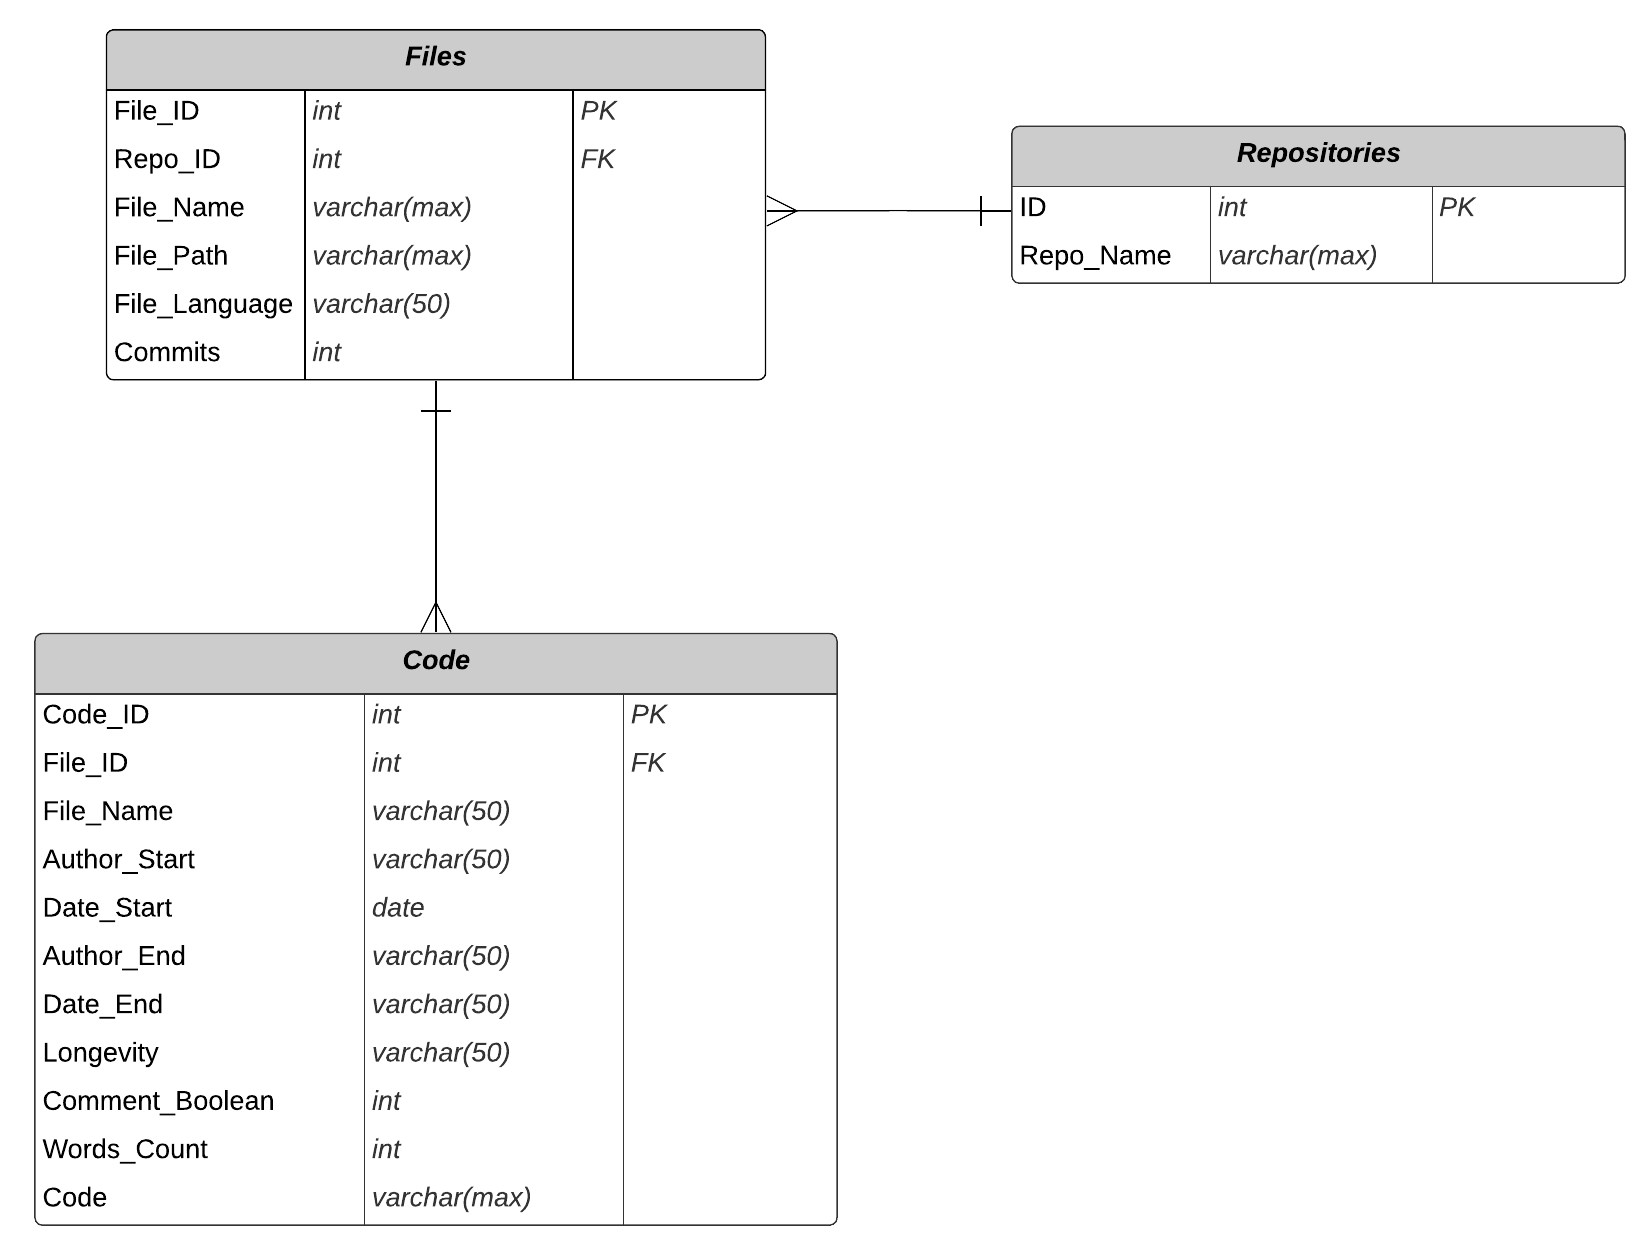
\includegraphics[width=14cm, keepaspectratio]{img/Diagrama_E-R.png}
  \caption{Diagrama de Entidad-Relación}
  \label{fig:entidad-relacion}
\end{figure}


\subsection{Procesado de datos}
\label{subsec:procesado}

Una vez recogidos y almacenados los datos, se realiza el procesamiento para prepararlos para el análisis. Esto puede implicar limpieza de datos (eliminación de valores atípicos, datos faltantes), normalización o estandarización de variables, selección de características relevantes y
transformación de datos según sea necesario.
Tenemos en cuenta diversas restricciones para que nuestro programa desarrolle su funcionamiento de manera eficiente. Teniendo en cuenta que el comando \textit{git blame} no es compatible con cualquier tipo de archivo, ajustamos el código
de manera que se eliminen del repositorio clonado los archivos con las siguientes extensiones [``.png", ``.jpg", ``.jpeg", ``.gif", ``.pdf", ``.exe", ``.dll", ``.ico", ``.db", ``.dat", ``.class", ``.o", ``.pyc", ``.mp3", ``.mp4", ``.wav", ``.avi", ``.bak", ``.tmp", ``.docx", ``.pptx", ``.zip",
``.tar.gz", ``.rar"]. También se eliminan los directorios [``node\_modules", ``vendor", ``Pods"], que se corresponden con directorios donde se organizan y gestionan todas las dependencias del proyecto, como bibliotecas y módulos de terceros. Otra necesidad importante ha sido
eliminar los archivos vacíos, es decir, aquellos que tienen un tamaño de 0 bytes. Estos archivos se utilizan comunmente para importar funciones y/o clases que se utilizan en otros módulos del proyecto, así como para marcar directorios como paquetes de Python, y producen errores
en la ejecución del código al no disponer de líneas de código para analizar. El directorio `.git' también ha sido descartado para el análisis pero teniendo en cuenta que no se puede eliminar, ya que conserva toda la información acerca del historial de revisiones del repositorio.

\\Una vez que se procede al análisis del repositorio clonado, se ha tenido en cuenta un manejo de todos los archivos en la codificación UTF-8, ya que permite un mayor manejo y procesado de los datos, así como menor dependencia de la detección automática consiguiendo así un menor flujo de trabajo.
Por lo que inicialmente se realiza una detección automática de la codificación de todos los archivos, pero con la finalidad de obtener cada uno de ellos en codificación UTF-8. Además, se han descartado líneas con más de 255 caracteres así como líneas en blanco, con la finalidad
de evitar errores al insertar los datos en la tabla denominada `Code'. 

\\También se realiza un procesado de datos teniendo en cuenta posibles funcionalidades a implementar en el futuro. Por lo que se identifica que cada línea de código sea un comentario o no, así como también se realiza un cálculo del número de palabras que tiene cada línea.

\subsection{Implementación de métricas y análisis}
\label{subsec:metricas}

A continuación, se desarrolla el objetivo más importante de este proyecto que consiste en el análisis de los datos. Mediante la implementación de distintas métricas, se pretenden estudiar distintos aspectos que resultan interesantes para analizar la evolución de los proyectos
FOSS\footnote{Free/Open Source Software} a lo largo de los años.
Tras la recopilación, revisión y limpieza de datos, se procede a la interpretación de los datos para la realización de un análisis estadístico, donde se han tenido en cuenta gran diversidad de factores como la antiguedad y/o tamaño del proyecto, el número de desarrolladores, la
complejidad que desarrolla, etc. Se realizan distintos análisis estadísticos tanto para el conjunto de todos los proyectos, como para cada uno de ellos de manera individual.

\subsubsection{Lenguajes de programación en uso}
\label{subsubsec:lenguajes}

Se ha estudiado para cada uno de los repositorios analizados, los distintos lenguajes de programación utilizados por los desarrolladores del proyecto. De manera que, haciendo un cálculo con todos los archivos del repositorio en cuestión, se obtienen los porcentajes de los lenguajes
de programación que tienen presencia dentro de cada proyecto. Se han tenido en cuenta todo tipo de lenguajes de programación, que se han obtenido mediante la biblioteca \textit{Pygments},  y si un archivo no corresponde a ningún lenguaje conocido, se ha clasificado como un archivo de
datos en un formato específico definido por el software que lo utiliza, y se ha denominado `Archivo de datos' o `Archivo binario'. Estos archivos, al no resultar relevantes, se han descartado del análisis estadístico.

\[\text{Porcentaje} \, \text{lenguaje} = \sum_{i=1}^{n} \left( \frac{\text{Archivo[lenguaje]}_i}{\text{Total} \, \text{de} \, \text{archivos[lenguaje]}} \right) \times 100\]

\subsubsection{Evolución de líneas pemanentes}
\label{subsubsec:lineas-vivas}

Resulta relevante estudiar el número de líneas que permanecen en la versión más actual del proyecto frente al momento de la creación del mismo, es decir, cuántas líneas permanecen intactas desde cualquier fecha pasada del proyecto. 
Esto puede aportar una estimación del esfuerzo de mantenimiento de cara a un futuro, debido a que un proyecto con una gran cantidad de líneas de código antiguas es más difícil de mantener, ya que puede que los autores 
hayan olvidado la razón de los cambios o incluso puede que ya ni siquiera formen parte del proyecto. Además, se puede observar qué proyectos se encuentran obsoletos en la actualidad, debido a que no hayan sufrido
modificaciones en un período largo de tiempo, así como también se pueden observar proyectos con una tendencia de trabajo constante con la finalidad de mantener el proyecto actualizado.

\\Entonces, se desarrollan dos métricas, una de ellas para obtener el número de líneas permanentes en la actualidad a lo largo de los años en valores absolutos, y otra para obtener los valores relativos respecto al tamaño total
del proyecto, y se aplican al total de repositorios seleccionados.

\[\text{Valor} \, \text{absoluto} = \sum_{i=1}^{n} \left( \frac{\text{Líneas} \, \text{vivas[repositorio][año]}_i}{\text{Líneas} \, \text{totales[repositorio]}} \right)\]

\[\text{Valor} \, \text{relativo} = \sum_{i=1}^{n} \left( \frac{\text{Líneas} \, \text{vivas[repositorio][año]}_i}{\text{Líneas} \, \text{totales[repositorio]}} \right) \times 100 \]


\subsubsection{Estabilidad del código}
\label{subsubsec:estabilidad-codigo}

Medir la estabilidad del código es posible gracias a una métrica denominada \textit{Tasa de Churn}. El análisis de esta métrica implica evaluar cuántas líneas de código han sido eliminadas en un período de tiempo específico.
Proporciona una medida de la actividad y volatilidad del código, resulta ser una herramienta muy útil para comprender la dinámica de cambio de un código a lo largo del tiempo. La finalidad de utilizar esta métrica en el proyecto
consiste en representar la \textit{tasa de Churn} por cada repositorio a lo largo de los años, comprobando así qué proyectos sufren una limpieza o mejora del código, o si por el contrario, contienen gran cantidad de código obsoleto.

\[\text{Tasa} \, \text{de} \, \text{Churn} = \sum_{i=1}^{n} \left( \frac{\text{Líneas} \, \text{eliminadas[repositorio][año]}_i}{\text{Líneas} \, \text{totales[repositorio]}} \right) \times 100 \]

\subsubsection{Frecuencia de cambios}
\label{subsubsec:commits}

Visualizar la frecuencia de cambios a lo largo del tiempo resulta útil para identificar períodos de actividad intensa o inactividad en el desarrollo del proyecto. Además, permite conocer las etapas del proyecto, ya que el desarrollo
inicial se corresponde con la etapa donde se lleva a cabo una alta frecuencia de cambios, pasando después a una etapa de estabilización con una frecuencia de cambios moderada, y siendo la etapa de mantenimiento aquella que tenga una
baja frecuencia de cambios. Conocer las etapas del proyecto puede ser útil para realizar una planificación y estimación del trabajo de cara a un futuro, ya que un proyecto con cambios frecuentes y regular resulta menos costoso en
términos de esfuerzo para implementar nuevas funcionalidades o mantenimientos.

\\La métrica utilizada nos permite visualizar la frecuencia de cambios, realizando un sumatorio del número de commits realizados en cada uno de los repositorios a lo largo de los años. 

\[\text{Número} \, \text{de} \, \text{commits}} = \sum_{i=1}^{n} \text{Commit[repositorio][año]}_i\]

\subsubsection{Número de colaboradores}
\label{subsubsec:numero-desarrolladores}

Otro dato relevante consiste en conocer la cantidad de colaboradores de un proyecto a lo largo de los años. Esto puede reflejar el crecimiento y la madurez del proyecto, ya que un aumento del número de desarrolladores
a lo largo del tiempo puede indicar un proyecto en expansión y cada vez más relevante, así como el caso contrario se traduce en una reducción del interés o fases críticas del proyecto. En proyectos de código 
abierto, la colaboración de múltiples desarrolladores indica un signo de confianza y relevancia en la comunidad. Por otro lado, un número alto de colaboradores se traduce en una diversidad de contribuciones, que aportan
diferentes perspectivas, habilidades y conocimientos, lo que puede conducir a un código más robusto con funcionalidades más variadas.

\\Se calcula el número de colaboradores teniendo en cuenta el creador de cada línea de código respecto al total de repositorios a lo largo de los años.

\[\text{Número} \, \text{de} \, \text{colaboradores}} = \sum_{i=1}^{n} \text{Colaborador[repositorio][año]}_i\]

\subsubsection{Evolución de la actividad de cada colaborador}
\label{subsubsec:actividad-desarrollador}

Conocer la actividad de cada colaborador del proyecto nos puede resultar interesante para una estimación de costes, ya que evaluando la contribución
individual se puede realizar una asignación de tareas más eficiente de acuerdo a las capacidades de cada colaborador. También resulta bastante útil conocer
conocer en qué momento ha desarrollado cada colaborador mayor protagonismo para recurrir a él en caso de tener que realizar posibles modificaciones respecto
a algo concreto desarrollado en esa etapa del proyecto, esto nos proporciona una mayor gestión de los recursos y una mejor planificación.
El hecho de visualizar las contribuciones individuales puede ayudar a mejorar el trabajo en equipo y el espíritu de colaboración.

\\La métrica para conocer la evolución de la actividad de cada colaborador del proyecto consiste en realizar un sumatorio del número de líneas
creadas por cada desarrollador del código para conocer los valores absolutos. Mientras que comparando con el número total de líneas de todos los colaboradores
del proyecto se calculan los valores relativos.

\[\text{Valor} \, \text{absoluto} = \sum_{i=1}^{n} \left( \frac{\text{Líneas} \, \text{vivas[colaborador][año]}_i}{\text{Líneas} \, \text{totales[colaborador]}} \right)\]

\[\text{Valor} \, \text{relativo} = \sum_{i=1}^{n} \left( \frac{\text{Líneas} \, \text{vivas[colaborador][año]}_i}{\text{Líneas} \, \text{totales[colaborador]}} \right) \times 100\]

\subsection{Representación gráfica de resultados}
\label{subsec:graficos}

Una vez que se han definido las métricas y los análisis estadísticos que resultan interesantes en este Trabajo Fin de Grado, se procede a una representación gráfica
de los resultados.


%%%%%%%%%%%%%%%%%%%%%%%%%%%%%%%%%%%%%%%%%%%%%%%%%%%%%%%%%%%%%%%%%%%%%%%%%%%%%%%%
%%%%%%%%%%%%%%%%%%%%%%%%%%%%%%%%%%%%%%%%%%%%%%%%%%%%%%%%%%%%%%%%%%%%%%%%%%%%%%%%
% RESULTADOS %
%%%%%%%%%%%%%%%%%%%%%%%%%%%%%%%%%%%%%%%%%%%%%%%%%%%%%%%%%%%%%%%%%%%%%%%%%%%%%%%%

\cleardoublepage
\chapter{Resultados}
\label{chap:resultados}

En este capítulo se presentan los resultados obtenidos tras la aplicación de la metodología descrita en el capítulo anterior, así como su evaluación para obtener las
conclusiones pertinentes.

\\Se han desarrollado varias fases con el objetivo de alcanzar la meta del proyecto, que incluyen la creación de una herramienta, la recopilación de datos y un análisis
estadístico. De esta manera, se busca comprender la evolución de los proyectos FOSS\footnote{Free/Open Source Software} alojados en GitHub.

\section{Descripción de los datos recopilados} 
\label{sec:datos-recopilados}

Los datos recopilados y almacenados en una base de datos, se han obtenido de una selección de repositorios siguiendo distintos criterios que concluyen en la tabla~\ref{tab:repositorios}.
En su posterior análisis, han participado archivos de todo tipo, encontrando así diversidad de datos que se observarán en las representaciones gráficas de los resultados.

\\En total, se han analizado 65.504.174 líneas de código de 11 repositorios de software libre alojados en GitHub, aplicándose las métricas que se presentan en los siguientes apartados.
Los resultados obtenidos, en forma de gráficas, proporcionan una comprensión integral de la evolución del software libre.

\section{Interpretación de los resultados} 
\label{sec:interpretación-resultados}

A continuación, tras recopilar y procesar los datos, así como aplicar la metodología correspondiente, se interpretan los resultados obtenidos del análisis gráficamente. Estas gráficas
muestran datos interesantes que reflejan el propósito final de este proyecto.

\subsection{Lenguajes de programación en uso}
\label{subsec:lenguajes}

En este análisis estadístico se ha evaluado cada repositorio individualmente, determinando el porcentaje de presencia de cada lenguaje de programación utilizado en cada uno de ellos. Se han generado 11
gráficas distintas como resultado, pero se enfocará la atención en las más relevantes.

\\En la figura~\ref{fig:lenguajes-perceval} se identifican 14 lenguajes de programación distintos en el repositorio \textit{grimoirelab-perceval}. Entre todos los lenguajes utilizados,
JSON, Markdown y Python son los más representativos, componeniendo alrededor del 70\% del código, siendo JSON el más predominante de los tres, con un 34\%.

\\Al analizar el repositorio de \textit{notebook}, se encuentran aún más lenguajes de programación, llegando a un total de 19, como se observa en la figura~\ref{fig:lenguajes-notebook}.
El lenguaje de programación JSON sigue siendo más dominante frente al resto, seguido de TypeScript. Otros lenguajes con una presencia significativa son CSS+Lasso, Django, Markdown y YAML,
que en conjunto forman alrededor del 12\% del código de programación.

\\Finalmente, la figura~\ref{fig:lenguajes-rath} muestra los lenguajes de programación utilizados en el repositorio \textit{rath}. En este caso, de entre los 15 lenguajes utilizados, Python y 
JavaScript son los predominantes con un 27\% y un 3\% respectivamente. Otros lenguajes con una notable presencia en el repositorio son JSON y Markdown.

\begin{figure}
  \centering
  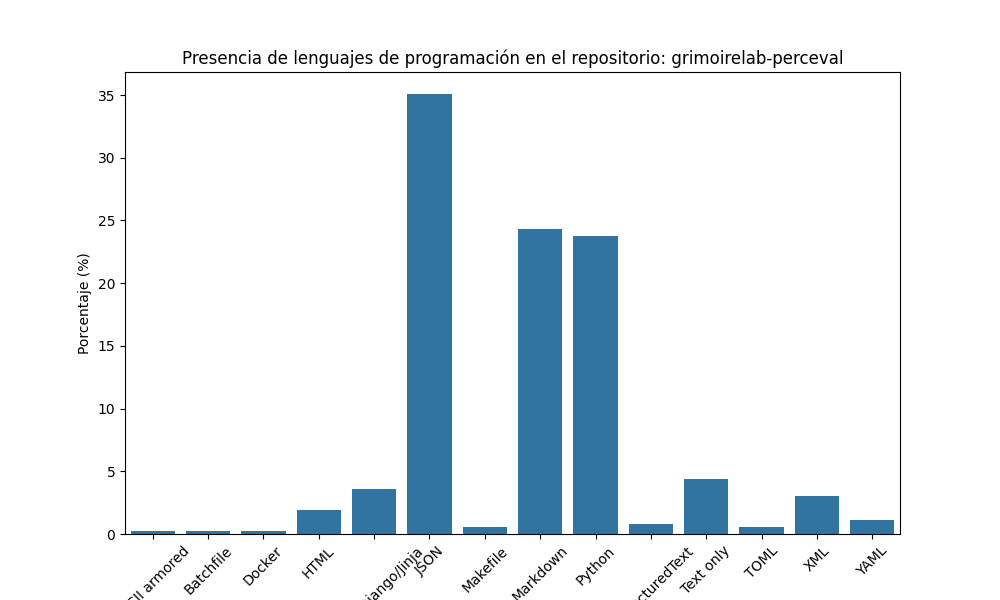
\includegraphics[width=16cm, keepaspectratio]{img/languages_grimoirelab-perceval.png}
  \caption{Lenguajes presentes en el repositorio Grimoirelab-Perceval}
  \label{fig:lenguajes-perceval}
\end{figure}

\begin{figure}
  \centering
  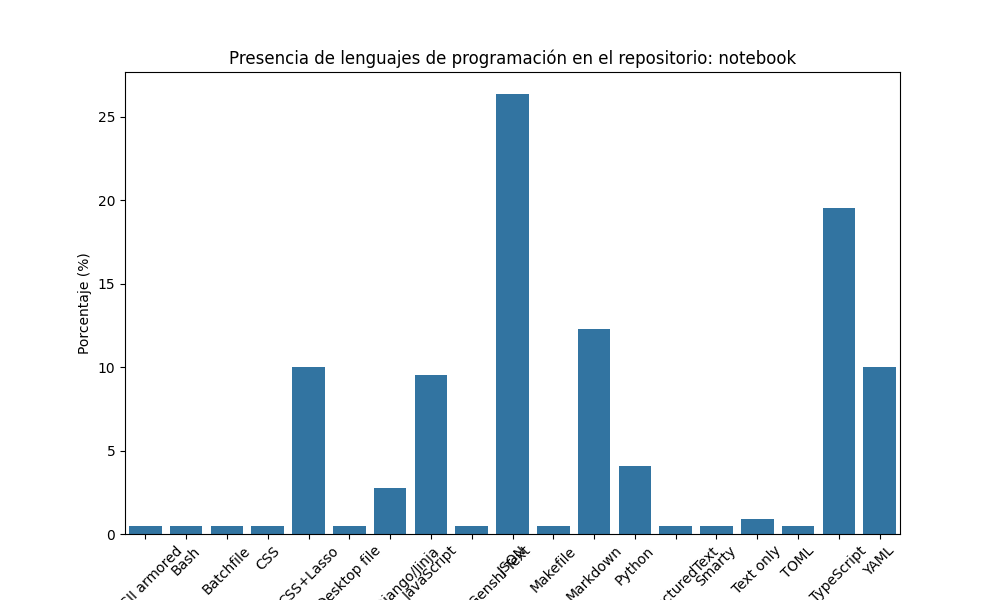
\includegraphics[width=16cm, keepaspectratio]{img/languages_notebook.png}
  \caption{Lenguajes presentes en el repositorio Notebook}
  \label{fig:lenguajes-notebook}
\end{figure}

\begin{figure}
  \centering
  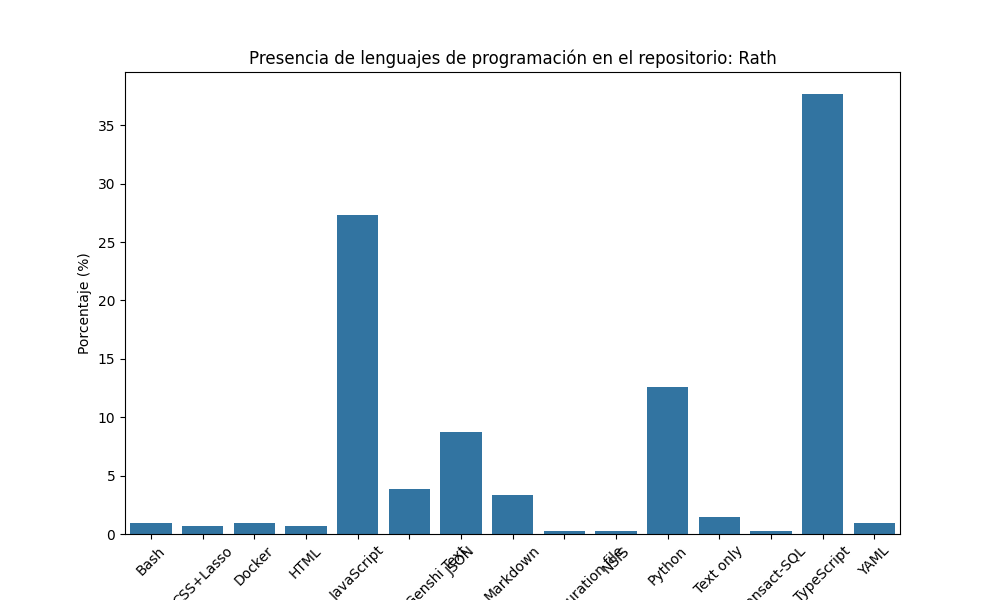
\includegraphics[width=16cm, keepaspectratio]{img/languages_rath.png}
  \caption{Lenguajes presentes en el repositorio Rath}
  \label{fig:lenguajes-rath}
\end{figure}

\subsection{Evolución de líneas pemanentes}
\label{subsec:líneas-permanentes}

\subsection{Estabilidad del código}
\label{subsec:estabilidad-código}

\subsection{Frecuencia de cambios}
\label{subsec:commits}

La figura~\ref{fig:grafica-commits} muestra gráficamente la evolución del número de commits en cada uno de los repositorios seleccionados a lo largo de los años. Se observa una etapa de
desarrollo desde el año 2008 hasta la actualidad, siendo el período de mayor actividad desde el año 2016 hasta el año 2024 .

\\El repositorio \textit{notebook} destaca como el proyecto más longevo, ya que comenzó su desarrollo en el año 2008 y sigue vigente en la actualidad.
Se identifica con un desarrollo constante aunque con períodos de baja actividad, y no ha experimentado su mayor etapa de desarrollo hasta el año 2019, cuando comienza a sufrir varios períodos intensos de actividad,
siendo el año 2023 el más destacable.

\\Por otra parte, el repositorio \textit{code-edit} es el proyecto más reciente, iniciando su desarrollo en 2022, y mostrando su mayor período de actividad durante ese mismo año.

\\Se observan repositorios de corta duración que hoy en día se encuentran en desuso y  no han tenido gran éxito dentro del mundo del software libre, como lo son \textit{nba-go} y \textit{ublhub}.
En contraste, los repositorios con larga trayectoria y un ritmo de actividad alto con una gran frecuencia de cambios a lo largo de los años, son \textit{luxon}, \textit{core}, \textit{notebook} y
\textit{Rath}. Estos proyectos, debido a su constante actualización, estiman menores costes en términos de esfuerzo para implementar nuevas funcionalidades o mantenimientos.

\\Los repositorios con menor frecuencia de cambios son \textit{Kap}, \textit{grimoirelab-perceval}, \textit{ant-design-pro} y \textit{ublhub}. Todos los mencionados, excepto \textit{ublhub}, siguen
manteniendo su actividad en la actualidad aunque no tengan una alta tasa de actividad.


\begin{figure}
  \centering
  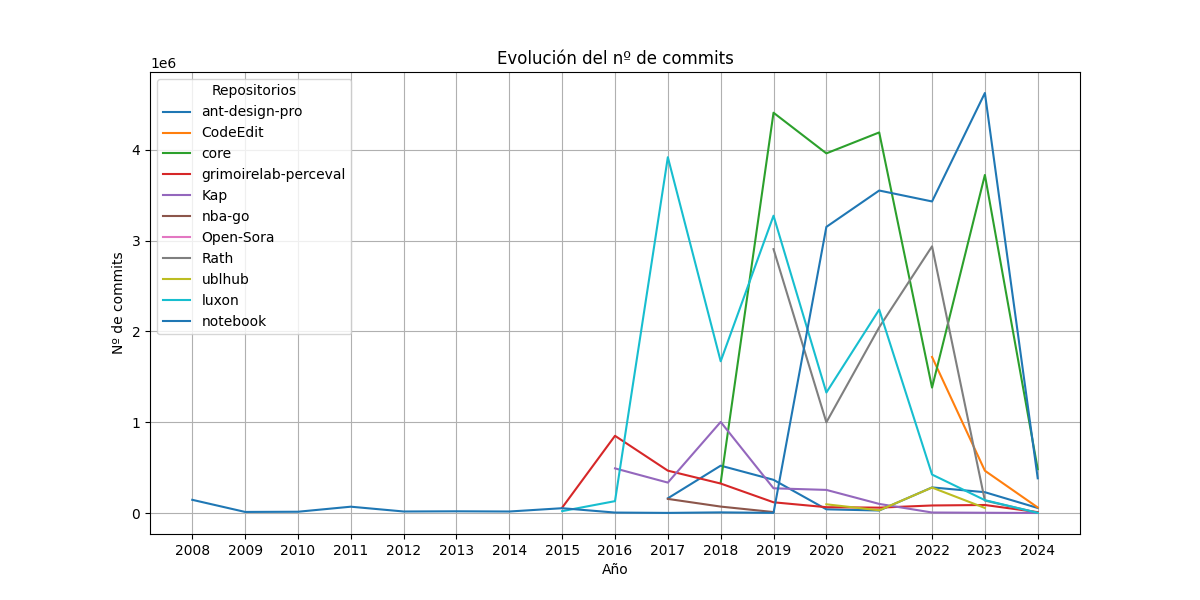
\includegraphics[width=16cm, keepaspectratio]{img/commits_graph.png}
  \caption{Evolución del número de commits a lo largo del tiempo}
  \label{fig:grafica-commits}
\end{figure}

\subsection{Número de colaboradores}
\label{subsec:número-colaboradores}

La figura~\ref{fig:grafica-colaboradores} muestra la cantidad de colaboradores de los proyectos seleccionados a lo largo de los años. Se identifican proyectos con un bajo número de colaboradores
durante su desarrollo, lo que se refleja en un bajo atractivo dentro de la comunidad de software libre. Entre estos proyectos destacan \textit{ublhub}, \textit{Kap} y \textit{nba-go}.

\\Por otro lado, algunos proyectos comiencan con un gran número de colaboradores, pero este número ha ido disminuyendo a lo largo de los años, indicando un decrecimiento del propio proyecto
pudiendo llegar incluso a desaparecer. Entre estos proyectos se encuentran \textit{grimoirelab-perceval}, \textit{luxon}, \textit{ant-design-pro} y \textit{CodeEdit}.

\\Los repositorios \textit{Notebook} y \textit{Rath} experimentaron un pico de desarrollo en el año 2022, alcanzando su número máximo de colaboradores en ese año. Sin embargo, no han logrado mantener
esta tendencia y en los próximos años el número de colaboradores disminuyó, volviendo a niveles similares a los de años anteriores.

\\El repositorio \textit{Core} destaca por sufrir los mayores picos de crecimiento en cuanto a colaboradores a lo largo de su desarrollo, lo que lo convierte en el proyecto más atractivo dentro de la
comunidad de software libre, llegando a contar con hasta 350 colaboradores.

\begin{figure}
  \centering
  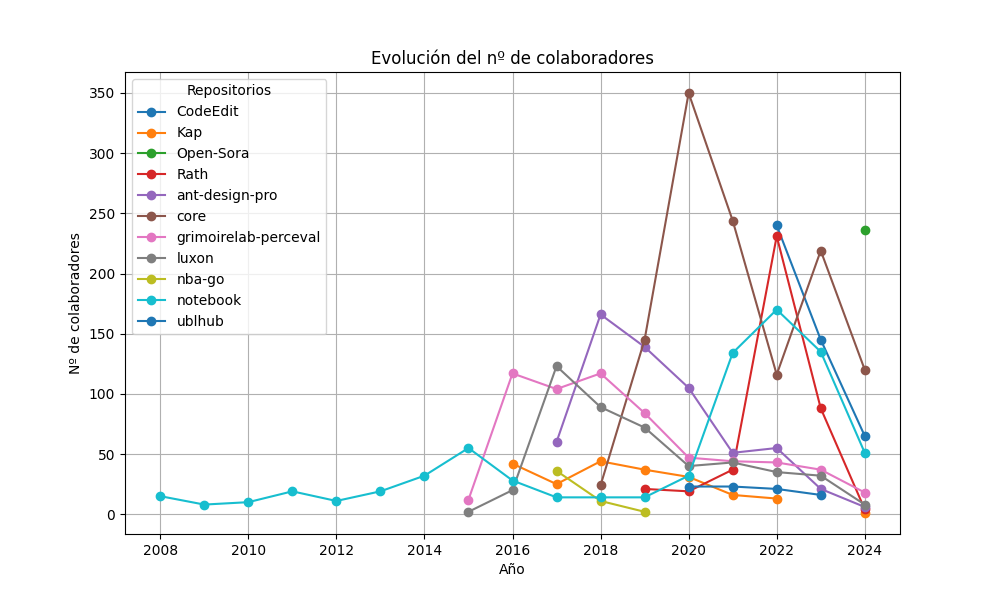
\includegraphics[width=16cm, keepaspectratio]{img/contributors_graph.png}
  \caption{Evolución del número de colaboradores a lo largo del tiempo}
  \label{fig:grafica-colaboradores}
\end{figure}

\subsection{Evolución de la actividad de cada colaborador}
\label{subsec:actividad-colaborador}

%%%%%%%%%%%%%%%%%%%%%%%%%%%%%%%%%%%%%%%%%%%%%%%%%%%%%%%%%%%%%%%%%%%%%%%%%%%%%%%%
%%%%%%%%%%%%%%%%%%%%%%%%%%%%%%%%%%%%%%%%%%%%%%%%%%%%%%%%%%%%%%%%%%%%%%%%%%%%%%%%
% CONCLUSIONES %
%%%%%%%%%%%%%%%%%%%%%%%%%%%%%%%%%%%%%%%%%%%%%%%%%%%%%%%%%%%%%%%%%%%%%%%%%%%%%%%%

\cleardoublepage
\chapter{Conclusiones}
\label{chap:conclusiones}

En este capítulo, se revisan los objetivos alcanzados y se abordan los problemas surgidos durante el desarrollo del proyecto. Además, se realiza una
reflexión sobre los conocimientos adquiridos tanto en este proyecto como a lo largo de mi formación académica, destacando su importancia para el
desarrollo del mismo. Como cierre a este capitulo, se presentan propuestas de mejoras futuras con el fin de perfeccionar y aumentar las funcionalidades
del programa desarrollado, lo que permitirá realizar un análisis más exhaustivo y enriquecer los resultados obtenidos.

\section{Consecución de objetivos}
\label{sec:consecucion-objetivos}

Teniendo en cuenta los resultados obtenidos y el análisis realizado, se puede concluir que los objetivos específicos de este Trabajo de Fin de Grado, establecidos
en el capítulo 2, se han cumplido de manera satisfactoria. Se ha llevado a cabo una exhaustiva búsqueda de los repositorios alojados en GitHub, identificando
y seleccionando aquellos que resultan más relevantes para nuestro Trabajo Fin de Grado, teniendo en cuenta su relevancia dentro de la plataforma y otros datos de interés para
su análisis posterior. Se ha desarrollado un proyecto de programación en Python que permite analizar el contenido de un repositorio, estudiando sus posibles limitaciones
y explorando en profundidad la utilidad del comando \textit{git blame}. Se han abordado y solucionado diversas restricciones relacionadas con algunos archivos o funcionalidades,
aportando al código más robustez. También se han solucionado problemas en relación al tamaño de la base de datos, puesto que se han encontrado dificultades al analizar 
repositorios de gran tamaño. Tras esto, se ha llevado a cabo una recopilación de los datos que resultan útiles para llevar a cabo un análisis estadístico, realizando un
procesado de los mismos para su posterior inserción en una base de datos. A partir de esta base de datos, se realiza una extracción de datos, evaluación e interpretación
de los mismos, presentando los resultados obtenidos de manera gráfica.

\\Con todo ello, se concluye que se ha logrado el objetivo general del proyecto, que consiste en estudiar la evolución de proyectos FOSS\footnote{Free/Open Source Software}
alojados en GitHub, obteniendo una comprensión integral de los cambios realizados a lo largo del tiempo, así como posibles patrones o tendencias  presentes en el código libre.

\section{Aplicación de lo aprendido}
\label{sec:aplicacion}

La aplicacion de los conocimientos y habilidades adquiridos durante mi formación académica en el Grado en Ingeniería en Sistemas Audiovisuales y Multimedia ha sido esencial para
la elaboración de este Trabajo de Fin de Grado. A continuación, se mencionan los aprendizajes que me permitieron llevar a cabo la extracción, tratamiento y clasificación de datos
para obtener como resultado el análisis de este proyecto.

\begin{itemize}
  \item \textbf{Informática I}. Esta asignatura fue mi primer contacto con el mundo de la programación. Me ha aportado conocimientos y habilidades para poder desarrollar mis primeros
  programas sencillos de manera efectiva, adquiriendo así las bases de la programación. 
  \item \textbf{Informática II}. Aparte de reforzar las bases de programación adquiridas, esta asignatura me ha aportado una nueva visión sobre los algoritmos y estructuras adaptados
  a los requisitos del software de comunicaciones. Además, al desarrollarse en el lenguaje de Python, me ha servido para adquirir mis primeros conocimientos del mismo.
  \item \textbf{Protocolos para la Transmisión de Audio y Vídeo en Internet}. En esta asignatura he seguido aprendiendo los conocimientos del lenguaje de programación Python, que han sido
  fundamentales para llevar a cabo el desarrollo de los scripts realizados en este proyecto. 
  \item \textbf{Estadística para Sistemas Audiovisuales}. Gracias a esta asignatura he adquirido la capacidad de definir modelos probabilísticos para resolver problemas de ingeniería.
  Por lo que he adquirido conocimientos de probabilidad y estadística que me han servido de utilidad en el proceso del análisis estadístico del proyecto.
\end{itemize}

\section{Lecciones aprendidas}
\label{sec:lecciones_aprendidas}

Durante la realización de este Trabajo de Fin de Grado, he tenido la oportunidad de adquirir diversos conocimientos sobre las herramientas utilizadas en un proyecto de análisis o minería
de datos, muchos de los cuales no había explorado con anterioridad ni durante mi formación académica. A continuación, se mencionan algunos de los aprendizajes más significativos que he
obtenido:

\begin{itemize}
  \item \textbf{Python}. La realización de este proyecto me ha permitido un mayor conocimiento de este lenguaje de programación, obteniendo nuevas habilidades
  y mejorando así mis capacidades para el desarrollo de código. Además, he adquirido conocimientos en muchas de las bibliotecas que utiliza, como por ejemplo \textit{subprocess} o
  \textit{matplotlib}, observando las posibilidades de desarrollo que nos aportan.
  \item \textbf{GitHub}. He entendido con mayor claridad el funcionamiento de la plataforma, así como del historial de revisiones. Además, he adquirido conocimientos
  sobre los distintos repositorios que se pueden encontrar en GitHub, ya que podemos observar repositorios muy diferentes y a su vez con grandes funcionalidades.
  \item \textbf{MySQL}. Dado que no tenía conocimientos acerca de bases de datos, he aprendido el significado de las mismas, centrándome en una base de datos relacional y
  en la forma en qué estructura los datos. Por lo que he aprendido a gestionar una base de datos relacional, llevando a cabo distintas tareas tanto de inserción como de
  extracción de datos.
  \item \textbf{LaTeX}. Otro conocimiento nuevo aprendido ha sido el sistema de composición de textos denominado LaTeX. Su aprendizaje no ha sido muy costoso, y me ha permitiendo
  estructurar la memoria de mi Trabajo de Fin de Grado de manera clara y organizada.
\end{itemize}

Otro ámbito donde he adquirido gran aprendizaje ha sido en mis aptitudes para realizar un proyecto de minería de datos. Este proyecto me ha permitido aumentar mi capacidad de análisis y de investigación,
sabiendo elegir y clasificar los repositorios y/o datos más importantes para utilizar en nuestro proyecto, y realizando un descarte de aquellos que no van a ser útiles para nuestro objetivo.
También he aprendido a desarrollar un proyecto de estas dimensiones, estructurando de manera clara toda la información a exponer y organizando las tareas y los tiempos de manera adecuada.
Otro aprendizaje a destacar es la resolución de problemas, puesto que he podido solventar distintos inconvenientes tanto del código como de la base de datos, haciendo posible la realización
final del proyecto.
Por último, cabe destacar mi aprendizaje redactando la información de este proyecto, desarrollando conceptos técnicos de la manera más clara posible, con el objetivo de un fácil entendimiento
de cara a posibles mejoras por diversos contribuidores en el futuro.

\section{Trabajos futuros}
\label{sec:trabajos_futuros}

Dado que ningún proyecto ni software se termina de manera definitiva, en esta sección se mencionan posibles ideas o mejoras que pueden implementarse en el futuro para adquirir un proyecto más
robusto y/o con nuevas funcionalidades.

\begin{itemize}
  \item \textbf{Estudio de un lenguaje de programación concreto}. Nuestro proyecto tiene en cuenta todos los posibles lenguajes de programación que se pueden encontrar en los repositorios alojados
  en GitHub, sin embargo podríamos modificar el programa de manera que solo tuviera en cuenta un lenguaje de programación en concreto. De esta forma, se podría estudiar la evolución y presencia de 
  este lenguaje en proyectos de código libre a lo largo de los años, observando si tiene relevancia en la plataforma o si se encuentra obsoleto frente a otros.
  \item \textbf{Evolución de las versiones de un mismo proyecto}. Un análisis que resulta interesante consiste en estudiar la evolución de las distintas versiones de un mismo proyecto a lo largo de los años.
  Se podría observar en que período de tiempo se ha dejado de desarrollar una versión antigua frente a la más nueva, así como si se comparten colaboradores entre versiones o si se da el caso contrario.
  \item \textbf{Estudio de proyectos de grandes dimensiones}. Estudiar la evolución de proyectos de gran relevancia conlleva enfrentarse a proyectos de grandes dimensiones, para los cuales tendríamos
  que aumentar la capacidad de la base de datos o incorporar múltiples bases de datos. Resolver los problemas que podamos encontrarnos y realizar mejoras para conseguir este objetivo resultaría muy
  interesante para estudiar proyectos que se encuentran en auge en la actualidad o que siempre han sido de vital importancia en el mundo de la programación. Además, esto ofrecería una mayor flexibilidad
  y escalabilidad al sistema.
  \item \textbf{Estudio de estructuras más utilizadas}. Puesto que se ha realizado un contador del número de palabras de cada línea de código, esto puede abrir puertas a un nuevo proyecto donde se estudie la
  presencia en mayor o menor grado de diversas estructuras. De esta manera, se puede estudiar la cantidad de veces que se utilizan listas o diccionarios en un archivo concreto, así como la presencia de
  sentencias de tipo If/Else o bucles. 
\end{itemize}

En resumen, este proyecto se plantea como una apertura a distintos estudios o implementaciones futuras, debido a que no se han desarrollado muchas investigaciones acerca de proyectos de código libre 
y abierto que utilicen un sistema de control de versiones.


%%%%%%%%%%%%%%%%%%%%%%%%%%%%%%%%%%%%%%%%%%%%%%%%%%%%%%%%%%%%%%%%%%%%%%%%%%%%%%%%
%%%%%%%%%%%%%%%%%%%%%%%%%%%%%%%%%%%%%%%%%%%%%%%%%%%%%%%%%%%%%%%%%%%%%%%%%%%%%%%%
% BIBLIOGRAFIA %
%%%%%%%%%%%%%%%%%%%%%%%%%%%%%%%%%%%%%%%%%%%%%%%%%%%%%%%%%%%%%%%%%%%%%%%%%%%%%%%%

\cleardoublepage

\nocite{*}

% Las siguientes dos instrucciones es todo lo que necesitas
% para incluir las citas en la memoria
\bibliographystyle{abbrv}
\bibliography{memoria}  % memoria.bib es el nombre del fichero que contiene
% las referencias bibliográficas. Abre ese fichero y mira el formato que tiene,
% que se conoce como BibTeX. Hay muchos sitios que exportan referencias en
% formato BibTeX. Prueba a buscar en http://scholar.google.com por referencias
% y verás que lo puedes hacer de manera sencilla.
% Más información: 
% http://texblog.org/2014/04/22/using-google-scholar-to-download-bibtex-citations/

\end{document}
